% Springer Nature manuscript template (sn-jnl)
% Compile with the official Springer Nature sn-jnl class and BibTeX.
\documentclass[pdflatex,sn-mathphys,Numbered]{sn-jnl}

\usepackage{graphicx}
\usepackage{booktabs}
\usepackage{tabularx}

\usepackage{array}
\usepackage{amsmath,amssymb}
\usepackage{multirow}
\usepackage{manyfoot}
\usepackage{url}
\usepackage{xcolor}
\usepackage{makecell}

\graphicspath{{resultats_inondations/}}

\begin{document}

\title[Multimodal flood dynamics and cropland exposure]{Multiyear Sentinel-1/2 and CHIRPS-Based Flood Dynamics and Potential Cropland Exposure in the Senegal River Valley}

\author*[1]{\fnm{Pape El Hadji Abdoulaye} \sur{Gueye}}\email{papeabdoulaye.gueye@uadb.edu.sn}
\author[1]{\fnm{Cherif Bachir} \sur{Deme}}
\author[1]{\fnm{Adrien} \sur{Basse}}
\author[1]{\fnm{Diery} \sur{Ngom}}
\affil*[1]{\orgdiv{UFR Sciences et Technologies de l'Information et de la Communication (SATIC)}, \orgname{Université Alioune Diop de Bambey}, \orgaddress{\city{Bambey}, \country{Senegal}}}

\abstract{
Floods threaten seasonal crops and livelihoods in the Senegal River Valley, yet satellite-detected water is not equivalent to verified crop damage or farmer income loss. We analyze Google Earth Engine exports for 2019--2024 (no 2018 observations are available), comprising 19,200 records from 200 repeated sites and Sentinel-1, Sentinel-2, CHIRPS, and historical-water covariates. Among five classifiers, the three highest-ranked by five-block spatial average precision are balanced Random Forest (0.220, SD 0.214), CatBoost (0.192, SD 0.178), and XGBoost (0.161, SD 0.136); however, persistence scores higher in spatial validation (AP 0.240, SD 0.125). On the joint 2024 future-and-unseen-site test, Random Forest reaches AP 0.379 versus 0.333 for persistence, but has a worse Brier score (0.037 versus 0.031); without contemporaneous Sentinel-1 predictors, AP falls to 0.202. Separate 10-m exports estimate general agricultural exposure of 1,936--8,827 ha per valid ten-day period; crop species are not distinguished. A conditional loss framework is described, but the available observations do not support estimates of crop-specific destruction, yield loss, or economic loss. Satellite exposure remains an unvalidated proxy, and independent flood, crop, and damage validation is required before operational use.
}

\keywords{Flood prediction, agricultural exposure, Sentinel-1, Sentinel-2, CHIRPS, Dynamic World, Google Earth Engine, Senegal River Valley}

\maketitle

\section{Introduction}
Floods can disrupt agricultural production through direct crop submergence, delayed field operations, erosion, and prolonged soil saturation. In semi-arid agricultural regions, however, the relationship between inundation and crop damage depends on flood duration, crop type, phenological stage, and local water management. Consequently, mapping flooded pixels alone does not quantify agricultural exposure, and agricultural exposure does not by itself prove crop damage or yield loss.

Remote-sensing studies in the Senegal River Valley have examined flood monitoring and flood-recession agriculture for decades \cite{sandholt2003,saarnak2003}. Recent work maps seasonal flood-recession cropland extent in the valley, while field-oriented analyses describe water constraints on flood-recession farming \cite{bruckmann2025,sall2020}. These studies motivate joint flood and agricultural-exposure assessment but do not make a satellite overlap map equivalent to measured crop damage or yield loss.

Despite this progress, three gaps remain relevant to the Senegal River Valley: (i) the need to examine flood dynamics across multiple seasons rather than a single season; (ii) the need to quantify the spatial overlap between potential inundation and candidate cropland; and (iii) the need for temporally honest prediction evaluation that separates earlier seasons from a later test season. This study addresses these gaps through a reproducible Google Earth Engine (GEE) workflow.

The objectives are to:
\begin{enumerate}
  \item construct a multiyear, multimodal point--time dataset from Sentinel-1, Sentinel-2, CHIRPS, and historical water information;
  \item map potential newly inundated surfaces and summarize their area and temporal frequency;
  \item assess which available products support quantification of potential cropland exposure and identify missing evidence;
  \item specify a conditional crop-loss calculation and illustrate its sensitivity without treating satellite exposure as observed damage;
  \item compare next-period classifiers using spatial, temporal, and joint space--time validation, with feature attribution.
\end{enumerate}

The term \emph{agricultural exposure} is used deliberately. Without independent agronomic or yield observations, the workflow cannot establish that an exposed field suffered a particular level of damage or production loss.

\section{Related work}
\subsection{Flood mapping from radar and optical imagery}
Sentinel-1 flood mapping ranges from threshold and change-detection processing to supervised classifiers and deep segmentation. Automated Sentinel-1 chains have reported event-dependent performance, and reviews emphasize the roles of training labels, sensors, and test-event design \cite{twele2016,bioresita2018,bentivoglio2022}. U-Net is an established segmentation architecture when spatially labeled training data are available \cite{ronneberger2015}.

Public reference resources such as Sen1Floods11 provide georeferenced Sentinel-1 water labels for algorithm development, while the Global Flood Database supports historical event mapping and exposure analyses \cite{bonafilia2020,tellman2021}. These resources illustrate the value of independent labels, but they do not validate the present point-period target: neither was co-registered and evaluated against the study sample here.

\subsection{Agricultural exposure and crop damage}
The relationship between inundation and crop impact depends on crop type, phenology, water management, and flood duration. For this reason, exposure maps should be distinguished from field-confirmed damage and yield outcomes. A relevant regional contribution is the mapping of flood-recession cropland extent in the Senegal River Valley \cite{bruckmann2025}; it is a cropland-mapping study, not a directly comparable next-period flood-classification benchmark.

The most relevant operational forecasting comparison is Google's river-flood system, which uses gauge-stage and rainfall sequences with year-held-out and extreme-event evaluation; its reported inundation-extent F1 values are not the same target as our next-dekad point labels \cite{nevo2022}. At global scale, an AI system predicts extreme river floods in ungauged watersheds at up to five days lead time and compares reliability against a global hydrological nowcast, again using a different target and reference framework \cite{nearing2024}. These are state-of-the-art context, not directly interchangeable score baselines. Spatially or temporally structured observations require blocked validation rather than random row splits \cite{roberts2017}.

\section{Methods}
\subsection{Study area, period, and sampling framework}
The study focuses on the Senegal River Valley (SRV), Senegal. The point source specified by the project is the pre-existing Earth Engine feature collection \texttt{projects/project37246/assets/points\_200\_vallee}, containing 200 point identifiers and coordinates. The available exports cover 2019--2024; no data for 2018 were present. Coordinates span $-16.4872$ to $-12.0523^\circ$ longitude and $14.1457^\circ$ to $16.8234^\circ$ latitude. All 200 identifiers recur in each year and each point has a single stable coordinate pair. The analysis covers 1 June--31 October in 2019--2024, represented by 16 ten-day periods per year. Each of the 96 year--period groups contains 200 records, yielding $200\times16\times6=19{,}200$ point--period rows. The point-generation code and sampling design were not included with the exports, so the sites are treated as a repeated sample, not a probability sample of the valley.

\begin{figure}[t]
\centering
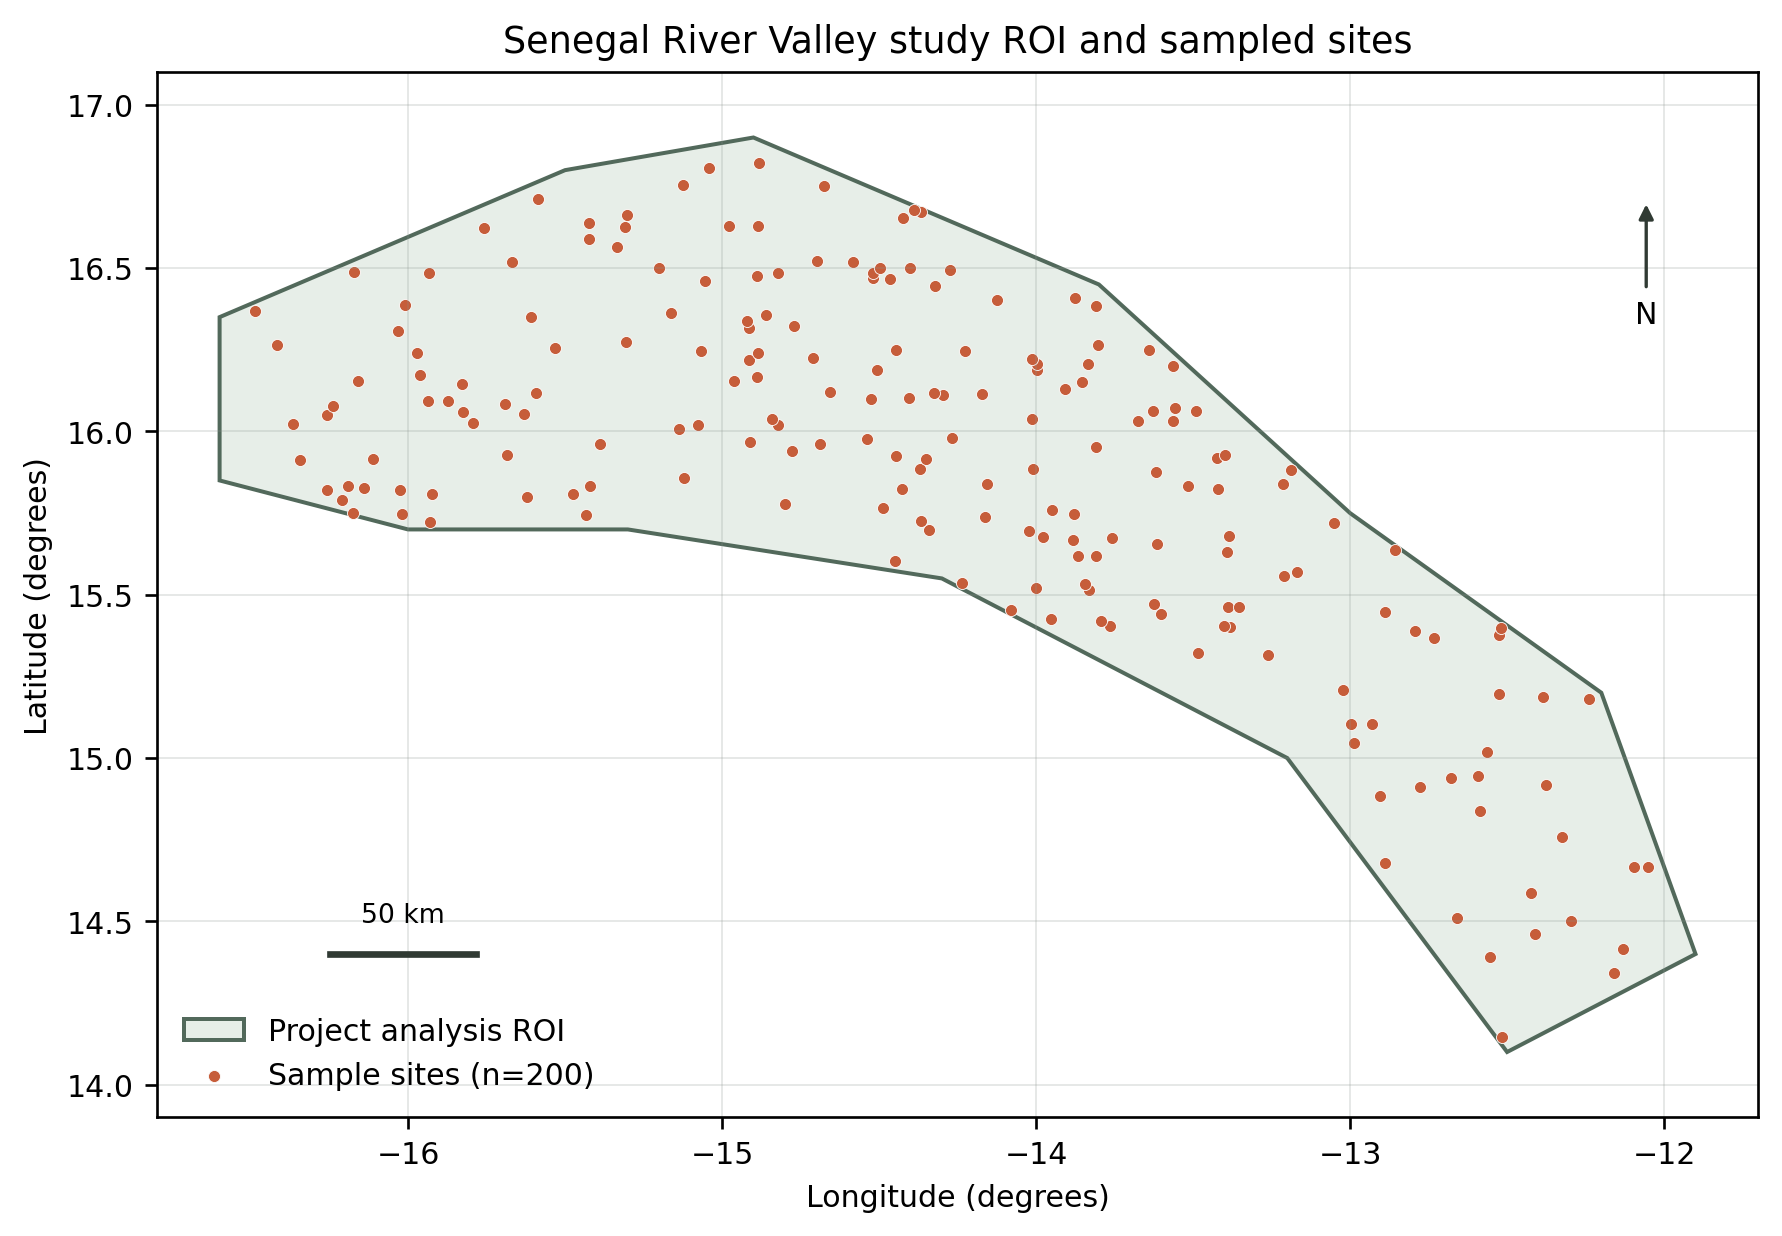
\includegraphics[width=0.76\linewidth]{13_zone_etude_sites.png}
\caption{Project-defined analysis ROI and the 200 sampled sites. The polygon is the study ROI used in the Google Earth Engine export, not an administrative boundary. River centerlines and administrative boundaries were not available in the project data and are therefore not shown.}
\label{fig:study-area}
\end{figure}

The primary key is $(\texttt{point\_id},\texttt{date\_debut})$; the export contains no duplicate keys. Temporal joins use the point identifier and period start rather than coordinate equality. Coordinate stability was checked within each identifier. The next-period label was compared with the within-point, within-year one-period shift of the current flood label; all 13,583 comparable pairs agree. The original extraction code, source rasters, and resampling parameters are not included, so pixel-level reprojection and the point-generation procedure cannot be independently reconstructed from the CSVs alone.

\subsection{Data products and harmonization}
The point--period export integrates Sentinel-1 GRD VV/VH backscatter and flood-screen indicators; Sentinel-2 Level-2A-derived NDVI, EVI, MSAVI, and NDWI; daily CHIRPS precipitation summaries; JRC Global Surface Water historical occurrence/extent; and Dynamic World crop-class probabilities used for candidate cropland. The sensors differ in pixel size, acquisition frequency, and cloud sensitivity: Sentinel-1/2 and Dynamic World are nominally 10 m products, JRC water is approximately 30 m, and CHIRPS is a substantially coarser precipitation grid. The Earth Engine export has sampled these products to common point--period records, but the exact reprojection and resampling settings are not available. All statistical results below use this delivered table, not a reconstructed raster stack. Product descriptions are available in the source literature \cite{funk2015,pekel2016,brown2022,torres2012,drusch2012,gorelick2017}.

\begin{table}[t]
\centering
\caption{Input products represented in the project export and their analytical roles.}
\label{tab:datasets}
\begin{tabular}{p{0.20\linewidth}p{0.31\linewidth}p{0.39\linewidth}}
\toprule
Product & Exported fields & Role and principal limitation \\
\midrule
Sentinel-1 GRD & VV, VH, water, dry reference, current/next label & Potential inundation proxy; not an independent flood reference. \\
Sentinel-2 L2A & NDVI, EVI, MSAVI, NDWI & Vegetation/water context; indices are missing when optical composites are unavailable. \\
CHIRPS daily & Ten-day, maximum-day, rainy-day and antecedent rainfall; SPI-labelled fields & Coarse precipitation covariates; no station-based local validation is supplied. \\
JRC Global Surface Water & Historical occurrence and maximum extent & Long-term water context, not an event-specific flood reference. \\
Dynamic World & Seasonal crop probability in the source workflow & Candidate cropland context; aggregated numeric exposure is available, but a validated per-pixel crop mask and crop-type labels are not archived. \\
\bottomrule
\end{tabular}
\end{table}

\subsection{Exploratory statistics and correlation tests}
Exploratory analysis includes variable types, unique values, missingness, descriptive statistics, annual and ten-day target prevalence, per-site recurrence conditional on valid observations, and period-level inundated-area summaries. Pearson product--moment ($r$) and Spearman rank ($\rho$) correlations are computed pairwise for numeric covariates and each flood target using available pairs. Nominal p-values and Benjamini--Hochberg q-values are retained in supplementary outputs for transparency, but are not used for confirmatory inference: repeated measurements at sites and temporal dependence violate independent-row assumptions, and multiplicity adjustment does not remove that dependence. Correlation is not interpreted causally. Highly collinear rainfall summaries are retained as candidate predictors but identified in the full correlation output.

\begin{figure}[t]
\centering
\begin{minipage}{0.48\linewidth}\centering
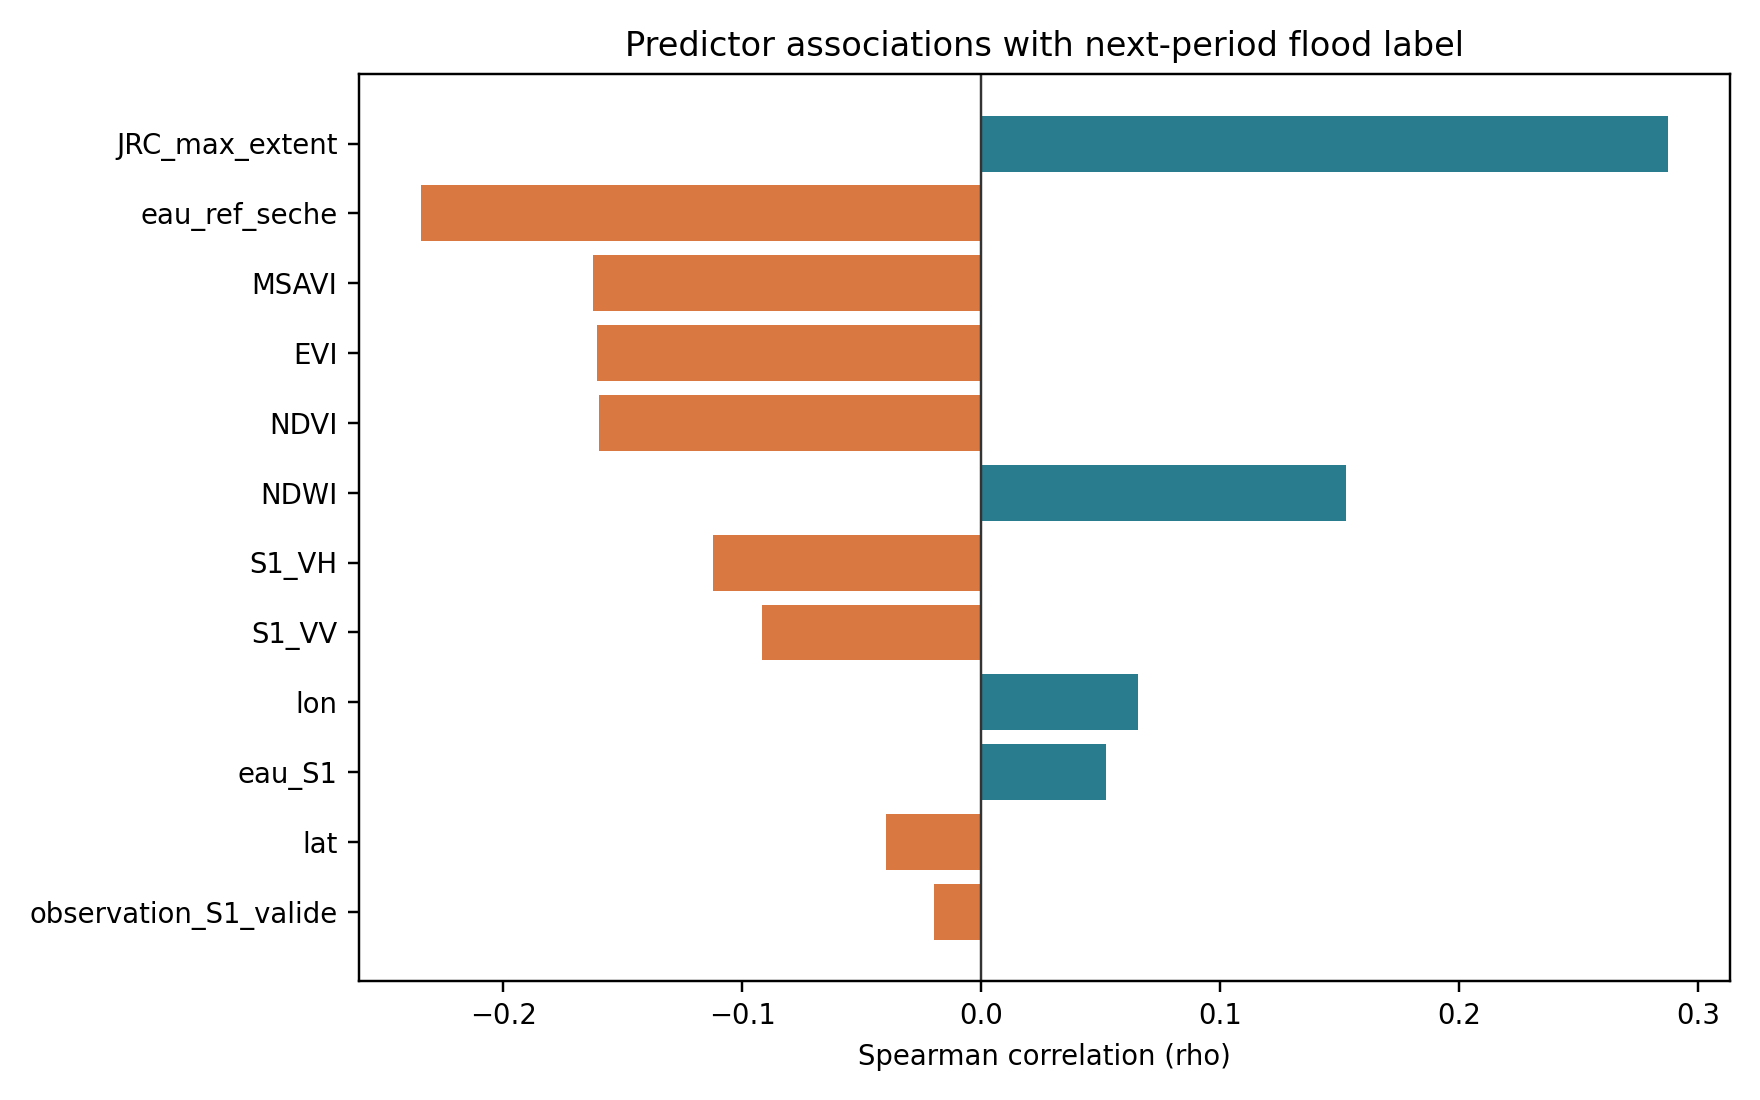
\includegraphics[width=\linewidth]{07_correlations_cible.png}
\end{minipage}\hfill
\begin{minipage}{0.48\linewidth}\centering
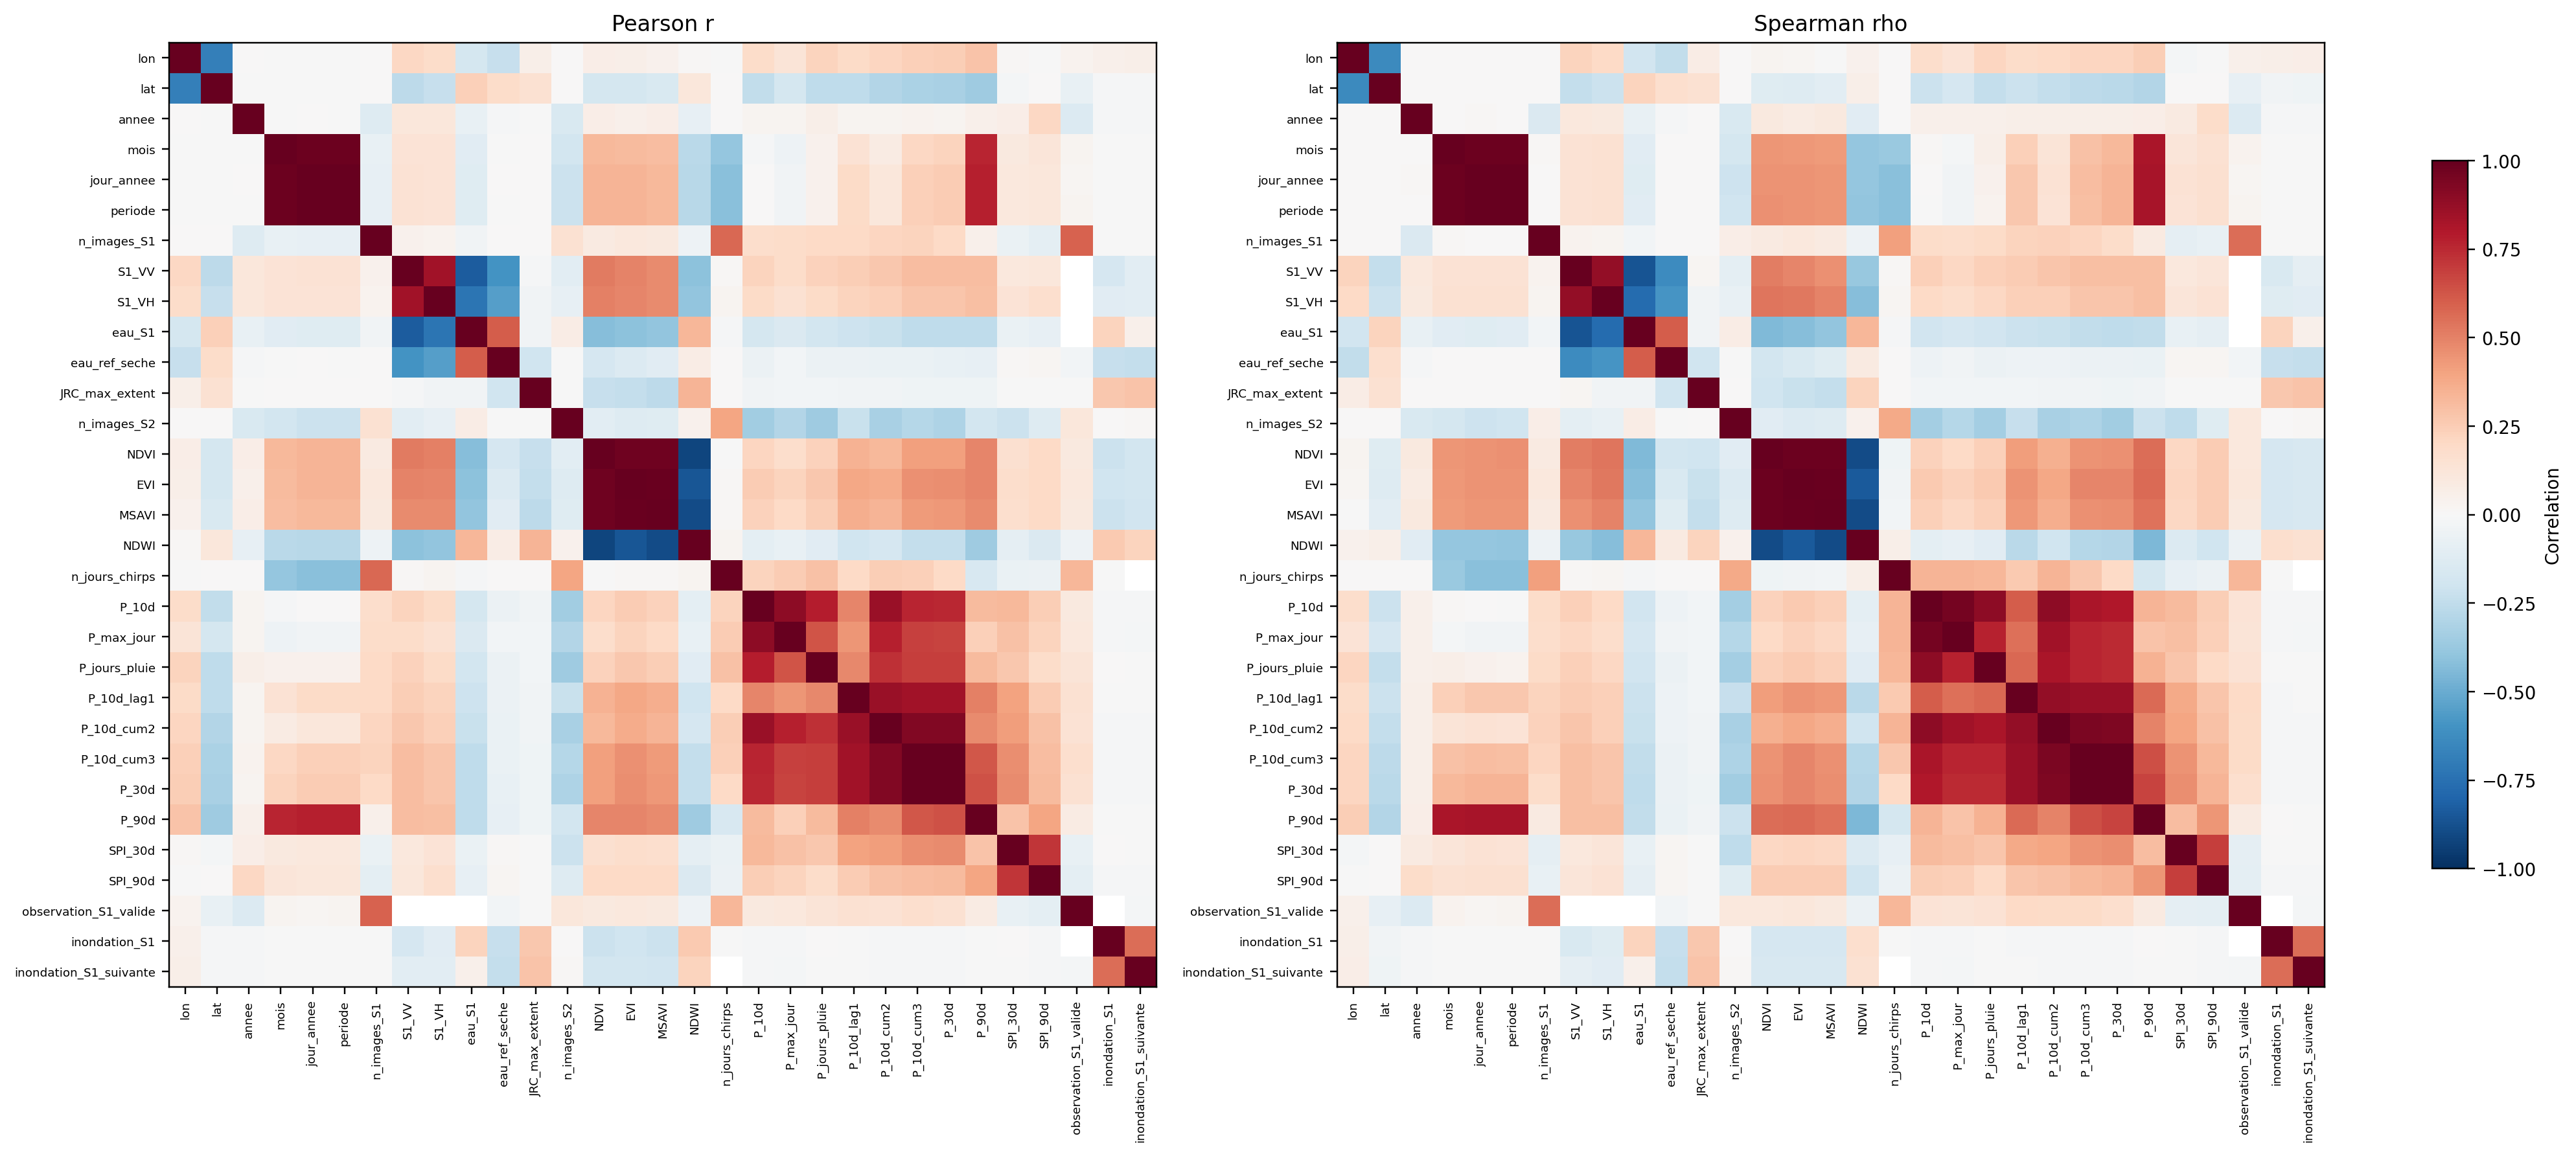
\includegraphics[width=\linewidth]{08_matrices_correlation.png}
\end{minipage}
\caption{Spearman associations of predictors with the next-period target (left) and full Pearson/Spearman correlation matrices (right). Pairwise sample sizes, p-values, and false-discovery-rate q-values are supplied in the CSV outputs.}
\label{fig:correlations}
\end{figure}

\subsection{Sentinel-1 observations and potential inundation}
Sentinel-1 GRD imagery is obtained from \texttt{COPERNICUS/S1\_GRD}. Images in IW mode with VV and VH polarizations are filtered to the study region and each ten-day period. Median composites are generated, and a spatial median filter is applied to reduce speckle. The VV backscatter is used for an initial potential-water screen:
\begin{equation}
W_{i,t} =
\begin{cases}
1, & VV_{i,t}<\tau_{\mathrm{VV}},\\
0, & VV_{i,t}\geq\tau_{\mathrm{VV}},
\end{cases}
\label{eq:water}
\end{equation}
where the initial threshold is $\tau_{\mathrm{VV}}=-16$ dB. This is an operational screening threshold, not a universally valid water/land boundary, and it should be tested against independent reference data.

For each year, a pre-season reference is generated from 1 March to 15 May. Let $W^{\mathrm{ref}}_{i,y}$ be the potential-water indicator derived from that reference. Potential newly inundated pixels are defined as
\begin{equation}
F_{i,t}=W_{i,t}\left(1-W^{\mathrm{ref}}_{i,y}\right).
\label{eq:flood}
\end{equation}
The label $F_{i,t}=1$ therefore indicates water detected in the current composite but not in the pre-season reference. It is not equivalent to independently confirmed flooding. Pixels without valid radar observations are treated as missing rather than as non-flooded.

The JRC Global Surface Water product (\texttt{JRC/GSW1\_4/GlobalSurfaceWater}) provides historical water occurrence and maximum extent. These layers are contextual covariates and are not interpreted as event-specific flood observations.

\subsection{Sentinel-2 vegetation and water indices}
Sentinel-2 Level-2A imagery is obtained from \texttt{COPERNICUS/S2\_SR\_HARMONIZED}. Scenes with reported cloud percentage below 40\% are retained, and the scene classification layer is used to mask cloud, shadow, defective, and no-data classes. Ten-day median composites are used to calculate NDVI, EVI, MSAVI, and NDWI:
\begin{align}
NDVI &= \frac{\rho_{B8}-\rho_{B4}}{\rho_{B8}+\rho_{B4}},\\
EVI &= 2.5\frac{\rho_{B8}-\rho_{B4}}{\rho_{B8}+6\rho_{B4}-7.5\rho_{B2}+1},\\
MSAVI &= \frac{2\rho_{B8}+1-\sqrt{(2\rho_{B8}+1)^2-8(\rho_{B8}-\rho_{B4})}}{2},\\
NDWI &= \frac{\rho_{B3}-\rho_{B8}}{\rho_{B3}+\rho_{B8}}.
\end{align}
Here, $\rho_{B2}$, $\rho_{B3}$, $\rho_{B4}$, and $\rho_{B8}$ denote scaled blue, green, red, and near-infrared reflectance. NDWI is treated as a complementary water-related indicator rather than definitive evidence of inundation. Optical missingness caused by clouds or absent acquisitions is preserved.

\subsection{CHIRPS precipitation and antecedent rainfall}
Daily precipitation is drawn from CHIRPS Daily (\texttt{UCSB-CHG/CHIRPS/DAILY}). The raw antecedent totals \texttt{P\_30d} and \texttt{P\_90d} are rolling sums through reference date $t$, excluding future daily observations:
\begin{equation}
P_n(t)=\sum_{d=t-n+1}^{t}r(d),\qquad n\in\{30,90\},
\end{equation}
where $r(d)$ is daily CHIRPS precipitation in millimetres. According to the GEE implementation specification supplied for this revision, the corresponding standardized fields use the mean and standard deviation of rolling totals for the same calendar day and month over 1991--2020:
\begin{equation}
Z_n(t)=\frac{P_n(t)-\mu_n(t)}{\sigma_n(t)},\qquad
\sigma_n(t)>\texttt{STD\_MIN\_WINDOW}=1\;\mathrm{mm},
\quad n\in\{30,90\}.
\end{equation}
The threshold masks pixels with standard deviation at or below 1 mm and can therefore create missing index values in low-variability locations or seasons. In the exported data these variables retain the legacy names \texttt{SPI\_30d} and \texttt{SPI\_90d}; mathematically they are z-score standardized rainfall anomalies, not conventional probabilistic SPI values. No Gamma or other probability-distribution fit is performed by the method described here. SPI-30 represents recent short-term rainfall anomalies, while SPI-90 represents a longer accumulated, seasonal rainfall context. Both describe antecedent rainfall only: neither is a flood observation nor sufficient to determine inundation, which also depends on discharge, upstream releases, topography, soils, drainage, and local water management.

The SPI source GEE script is not present in the project folder; the details above document the implementation specification supplied for this revision and could not be independently checked against executable SPI code. In the delivered CSV, \texttt{SPI\_30d} and \texttt{SPI\_90d} have 222 and 216 missing values, respectively, and no $-9999$ sentinel values. Missing predictors are imputed within each training fold. The fixed 1991--2020 reference includes 2020 data for some earlier sample dates; while the rolling total itself excludes rainfall after $t$, a strictly prospective analysis of pre-2020 origins would need a climatological reference limited to years available at each origin.

\subsection{Candidate agricultural mask}
This study does not classify or distinguish rice, maize, millet, sorghum, or other crop species. It uses only the general \texttt{crops} class-probability band in Google Dynamic World (\texttt{GOOGLE/DYNAMICWORLD/V1}) to identify candidate agricultural surfaces. For each year, the seasonal mean probability over 1 June--1 November is thresholded at \texttt{CROP\_PROBABILITY\_THRESHOLD}=0.30 to create a general agricultural mask:
\begin{equation}
C_{p,y}=\mathbb{I}\left(\overline{q}^{\,\mathrm{crop}}_{p,y}\geq0.30\right),
\end{equation}
where $\overline{q}^{\,\mathrm{crop}}_{p,y}$ is the seasonal mean probability and $\mathbb{I}$ is the indicator function. In the available agricultural GEE export, the corresponding internal objects are named \texttt{cropProbability}, \texttt{cropMask}, and \texttt{cropFlooded}; the CSV reports general fields such as \texttt{superficie\_agricole\_inondee\_ha}. The names \texttt{proba\_culture}, \texttt{zone\_agricole}, and \texttt{cultures\_inondees} are not fields in this script or its exports. Dynamic World probabilities indicate a broad land-cover class, not crop species, crop calendar, verified parcels, or crop destruction. The resulting area is general satellite-derived agricultural exposure only and is conditional on the mask and its classification accuracy.

\subsection{Area and temporal frequency of potential inundation}
For a binary inundation mask $F_{p,t}$ and pixel area $a_p$ in square metres, total potential inundated area for period $t$ is calculated as
\begin{equation}
A^{\mathrm{flood}}_t=\frac{1}{10^4}\sum_p a_pF_{p,t},
\end{equation}
where only valid radar pixels are included. The potential agricultural area exposed is
\begin{equation}
A^{\mathrm{crop,flood}}_t=\frac{1}{10^4}\sum_p a_pF_{p,t}C_{p,y}.
\end{equation}
The denominator for the exposed-cropland percentage includes only candidate crop pixels observed by valid radar in the corresponding period:
\begin{equation}
R^{\mathrm{crop}}_t=100\,
\frac{A^{\mathrm{crop,flood}}_t}{A^{\mathrm{crop,observed}}_t}.
\end{equation}
A missing radar pixel is not counted as a non-flooded pixel. In the sampled table, the current-period point label is exported as \texttt{inondation\_S1}; the next-period target \texttt{inondation\_S1\_suivante} is the within-year next-dekad label, with the terminal dekad lacking a next-period target. Seasonal frequency maps are computed from the number of valid periods with potential inundation divided by the number of valid radar observations at each pixel. Agricultural exposure is the intersection of the general Dynamic World \texttt{cropMask} and Sentinel-1-derived flood mask, restricted to valid radar observations; it is not a crop-specific inundation or destruction product.

\subsection{Conditional crop-production and gross-value loss model}
Satellite-derived inundated area is an exposure measure, not a crop-loss observation. For crop $i$, $S_i$ is the hectares of crop actually affected during the relevant crop stage, $R_i$ is its expected yield in tonnes per hectare, $P_i$ is its farm-gate price in FCFA per tonne, and $D_i\in[0,1]$ is the fraction of expected production destroyed. $Q_i$ denotes production loss in tonnes, $L_i$ denotes gross production value lost in FCFA, and $n$ is the number of crop types. Conditional on independently identifying crop-specific affected area and damage, we calculate
\begin{align}
Q_i &= S_iR_iD_i, & Q_{\mathrm{total}} &= \sum_{i=1}^{n}S_iR_iD_i,\\
L_i &= S_iR_iP_iD_i, & L_{\mathrm{total}} &= \sum_{i=1}^{n}S_iR_iP_iD_i.
\end{align}
The dimensions are $\mathrm{ha}\times(\mathrm{t}/\mathrm{ha})=\mathrm{t}$ for $Q_i$ and $\mathrm{ha}\times(\mathrm{t}/\mathrm{ha})\times(\mathrm{FCFA}/\mathrm{t})=\mathrm{FCFA}$ for $L_i$. $D_i=1$ represents total destruction; values 0.75, 0.50, and 0.25 represent corresponding partial losses. The area $S_i$ must refer to productive crop area with observed damage, not all water-detected pixels or all Dynamic World crop candidates. Flood-recession and seasonal floods can also support production; they must not be assigned a negative economic impact without a crop-specific counterfactual.

For an illustrative rice calculation only, the provisional inputs are 5.5 t/ha for paddy-rice yield and 160,000 FCFA/t for paddy price. They imply a gross output value of 880,000 FCFA/ha before costs. These values are scenario inputs provided for this analysis, not verified or universal Senegalese statistics; the price is for paddy, not milled white rice, and must be replaced with campaign-, location-, and quality-specific evidence before interpreting results. A 20\% range around each input (4.4--6.6 t/ha and 128,000--192,000 FCFA/t) is used only as a transparent sensitivity assumption. The satellite exports do not identify rice parcels or field-level destruction, so this model is not used to report observed annual losses.

\begin{table}[t]
\centering
\caption{Provisional rice parameters used only for illustrative scenarios.}
\label{tab:rice-parameters}
\begin{tabular}{p{0.29\linewidth}p{0.19\linewidth}p{0.18\linewidth}p{0.25\linewidth}}
\toprule
Parameter & Value & Unit & Evidence status \\
\midrule
Reference paddy yield, $R_{\mathrm{rice}}$ & 5.5 & t/ha & Provisional assumption; source and campaign to be verified \\
Paddy price, $P_{\mathrm{rice}}$ & 160,000 & FCFA/t & Indicative 2025 assumption; not an official universal price \\
Gross value at reference yield & 880,000 & FCFA/ha & Derived as $R_{\mathrm{rice}}P_{\mathrm{rice}}$ \\
\bottomrule
\end{tabular}
\end{table}

For illustration only, if a separately verified 1,500-ha rice area were fully destroyed, the provisional assumptions yield $Q=1{,}500\times5.5\times1=8{,}250$ t and $L=8{,}250\times160{,}000=1{,}320{,}000{,}000$ FCFA. At an assumed destruction fraction $D=0.50$, these become 4,125 t and 660,000,000 FCFA. These calculations are hypothetical and are not an application of the satellite-derived general agricultural area.

```latex
\begin{table}[t]
\centering
\caption{Illustrative rice-loss scenarios for a hypothetical affected area of 1,500 ha. Low/high yield and price values are $\pm20\%$ sensitivity assumptions around provisional inputs; destruction fractions are scenario assumptions. None is an observed loss.}
\label{tab:rice-loss-scenarios}
\small
\setlength{\tabcolsep}{3pt}
\renewcommand{\arraystretch}{1.15}
\begin{tabularx}{\textwidth}{@{}X c c c c r@{}}
\toprule
Scenario &
\makecell{Yield\\(t/ha)} &
\makecell{Paddy price\\(FCFA/t)} &
$D$ &
\makecell{Production\\lost (t)} &
\makecell{Gross value\\lost (FCFA)} \\
\midrule
Optimistic hypothesis & 4.4 & 128,000 & 0.25 & 1,650 & 211,200,000 \\
Central hypothesis & 5.5 & 160,000 & 0.50 & 4,125 & 660,000,000 \\
Pessimistic hypothesis & 6.6 & 192,000 & 1.00 & 9,900 & 1,900,800,000 \\
Reference, total destruction & 5.5 & 160,000 & 1.00 & 8,250 & 1,320,000,000 \\
\bottomrule
\end{tabularx}
\end{table}
```

\begin{table}[t]
\centering
\caption{One-at-a-time sensitivity for the same hypothetical 1,500 ha. Other parameters are held at reference values ($R=5.5$ t/ha, $P=160{,}000$ FCFA/t, $D=0.50$). Ranges are assumptions, not measured confidence intervals.}
\label{tab:rice-loss-sensitivity}
\small
\begin{tabular}{p{0.20\linewidth}p{0.24\linewidth}p{0.25\linewidth}p{0.25\linewidth}}
\toprule
Varied factor & Low / base / high & Production lost (t) & Gross value lost (million FCFA) \\
\midrule
Yield (t/ha) & 4.4 / 5.5 / 6.6 & 3,300 / 4,125 / 4,950 & 528 / 660 / 792 \\
Paddy price (FCFA/t) & 128,000 / 160,000 / 192,000 & 4,125 / 4,125 / 4,125 & 528 / 660 / 792 \\
Destruction fraction $D$ & 0.25 / 0.50 / 1.00 & 2,062.5 / 4,125 / 8,250 & 330 / 660 / 1,320 \\
\bottomrule
\end{tabular}
\end{table}

\subsection{Next-period prediction target and leakage control}
To prepare a forecasting dataset, the candidate target is the potential-inundation indicator for the next ten-day period:
\begin{equation}
Y_{i,t+1}=F_{i,t+1}.
\end{equation}
The last period of each season has no next-period label and is excluded from supervised evaluation. The primary full-feature model is a one-dekad-ahead prediction of a Sentinel-1-derived proxy conditional on current-dekad observations; current-period VV/VH and water status are therefore available predictors but are not independent evidence of flood truth. We compare this model with persistence and report a sensitivity model excluding all contemporaneous Sentinel-1 predictors. The latter is the more conservative test of whether non-radar context contributes predictive signal. Neither setup is described as an independently validated flood forecast.

The chronological evaluation uses 2019--2023 for model development and 2024 as a held-out test season. The rolling rainfall totals use observations only through their forecast-origin date. However, the fixed 1991--2020 climatological reference includes 2020 observations for some earlier sample dates; the 2024 test is after this reference period, but strictly prospective analyses at pre-2020 origins would require a reference restricted to years available at each origin. If independent flood labels are unavailable, the task is prediction of Sentinel-1-derived potential inundation, not independently verified flooding.

\subsection{Model candidates and evaluation}
Five tabular classifiers are compared: a prevalence dummy baseline, class-balanced logistic regression, class-balanced Random Forest (400 trees), XGBoost, and CatBoost. The three highest-ranked non-baseline classifiers by spatial-validation average precision are reported as candidate models, not as operationally validated winners. The primary predictors include coordinates, calendar variables, radar and optical features, historical water extent, precipitation summaries, and radar-observation validity. The entirely missing \texttt{NDVI\_ref}, identifiers, current flood label, next-period target, and \texttt{eau\_ref\_seche} are excluded; the latter contributes directly to label construction. Hyperparameters are fixed rather than tuned, so model rankings are exploratory. We also evaluate two simple references: persistence (current-period label carried forward) and the historical target frequency at each site, computed from training years only. A Sentinel-1 ablation removes current-period VV/VH, water, image count, and radar-validity predictors. At threshold 0.5, precision, recall, F1, balanced accuracy, ROC-AUC, average precision, and Brier score are reported.

Generalization is examined in three ways. First, five-fold grouped spatial validation is run on 2019--2023: the 200 sites are partitioned into five coordinate-based K-means blocks, and each fold holds out all records from one block. The leading candidate is selected by mean fold average precision, with per-block variability reported. Second, models and baselines are trained on 2019--2023 and evaluated on 2024, where sites recur from training. Third, a joint space--time test predicts 2024 records only for held-out spatial blocks, with those blocks excluded from all training years. The blocks are clusters, not buffered partitions, and neither this evaluation nor the spatial folds establish valley-wide transferability. All targets remain Sentinel-1-derived proxies.

SHAP values are calculated for the model selected by spatial validation, on a random sample of up to 600 labeled 2024 observations with a training-derived background sample. Mean absolute SHAP values rank global contribution magnitude; summary and dependence plots display contribution direction and distribution. SHAP is an attribution of the fitted model, not a causal effect, and correlated predictors can share or redistribute importance \cite{lundberg2017}.

The 96 agricultural period records support descriptive general agricultural-exposure summaries; they do not support fitting or validating a crop-impact model. No crop-specific affected area, observed destruction fraction, yield, campaign-specific price, or household-income outcome is included in the exports, so no annual production or financial loss is estimated. The preceding rice examples are methodological scenarios only. Count models, event-level area forecasting, and image segmentation remain future work, not results of this study.

\subsection{Validation and uncertainty}
The VV threshold, dry-reference dates, Dynamic World crop-probability threshold, and spatial scale can influence estimated areas. Sensitivity analysis should vary these settings and compare mapped outputs with independent flood references where available. Spatially nearby points are not independent replicates; where feasible, validation should additionally group locations spatially. Cloud gaps, missing radar acquisitions, mixed pixels, seasonal water, irrigation, and land-cover classification errors are documented as sources of uncertainty.

\section{Results}
\subsection{Dataset completeness and temporal coverage}
The main export contains 19,200 rows for 200 sites, six years, and 16 ten-day periods per year. Each year--period group contains 200 records, site coordinates are constant within identifier, and no duplicate $(\texttt{point\_id},\texttt{date\_debut})$ keys were found. There are 14,519 valid current flood labels (3.73\% positive) and 13,583 valid next-period targets (3.76\% positive); 29.26\% of next-period labels are missing. Sentinel-1 fields and current labels are missing in 24.38\% of rows, optical indices in 26.83\%, and CHIRPS summaries in 0.50--1.16\%. The \texttt{NDVI\_ref} field is entirely missing. The next-period target was checked against a within-year, within-site one-period shift of the current flood label; all 13,583 comparable labels aligned.

\begin{figure}[t]
\centering
\begin{minipage}{0.48\linewidth}\centering
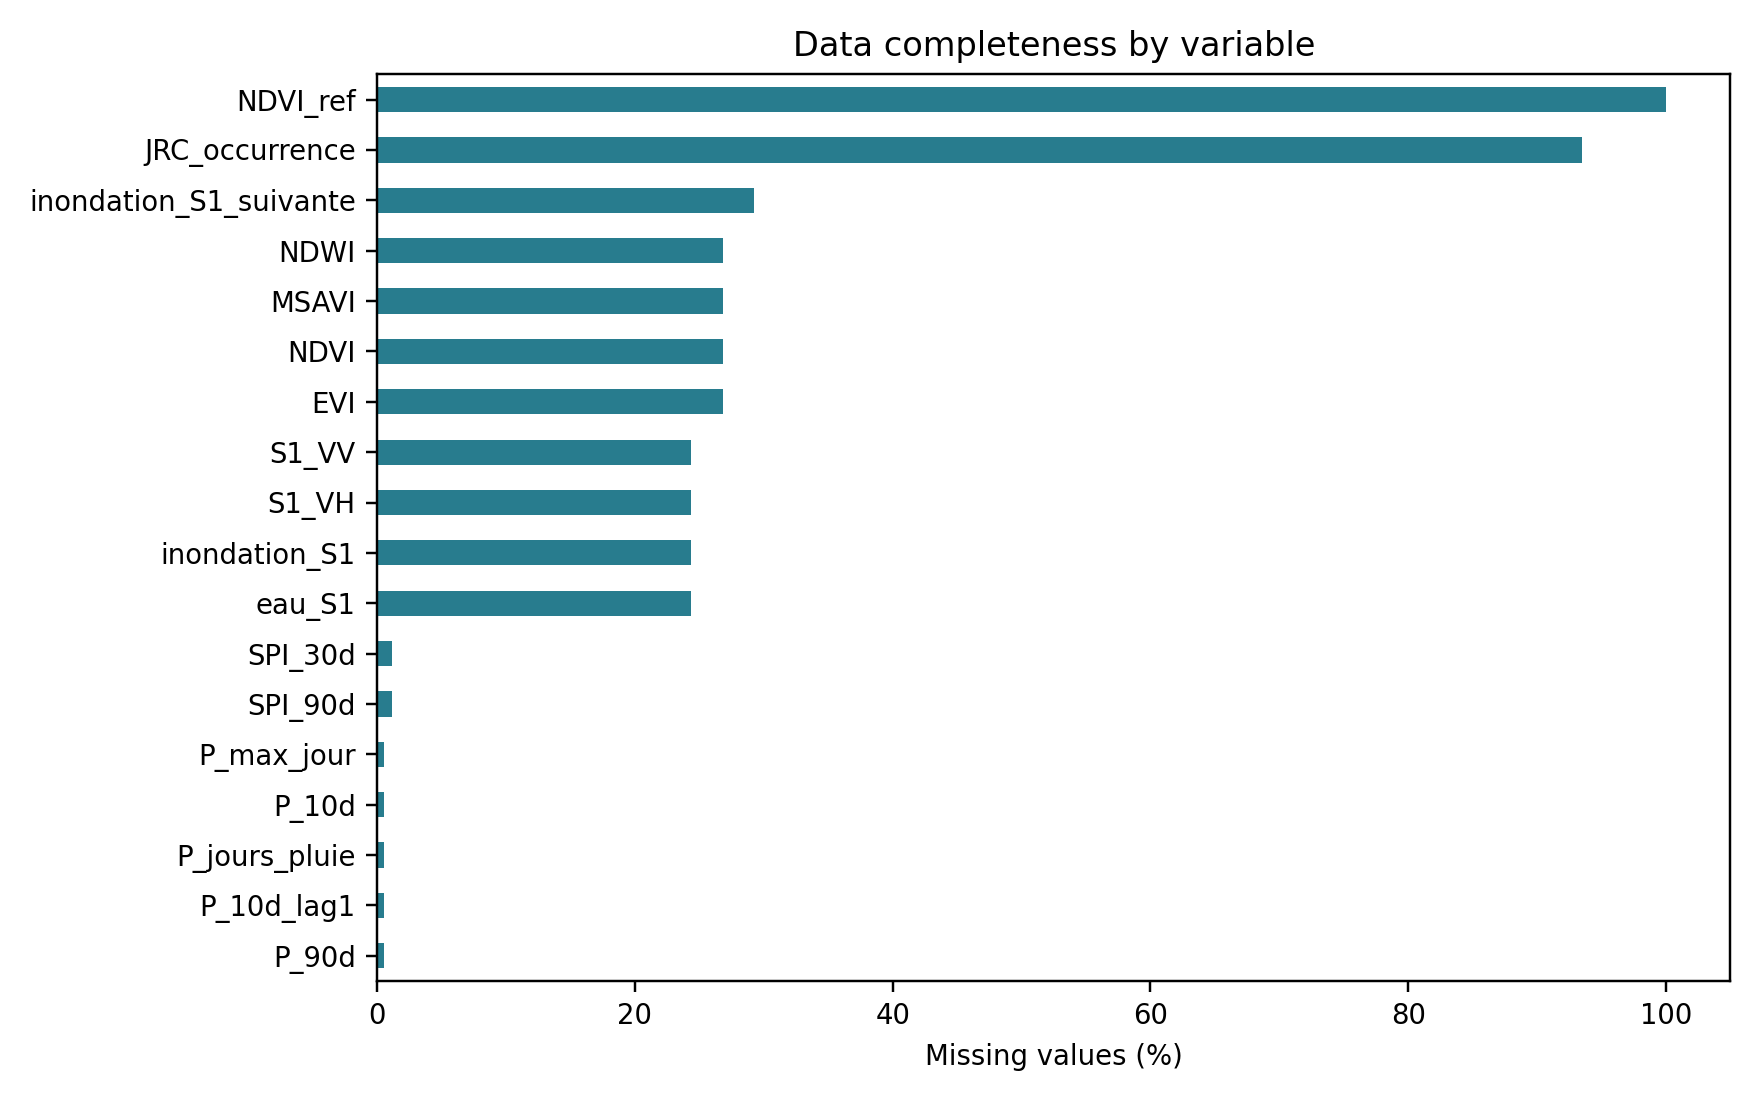
\includegraphics[width=\linewidth]{01_missingness.png}
\end{minipage}\hfill
\begin{minipage}{0.48\linewidth}\centering
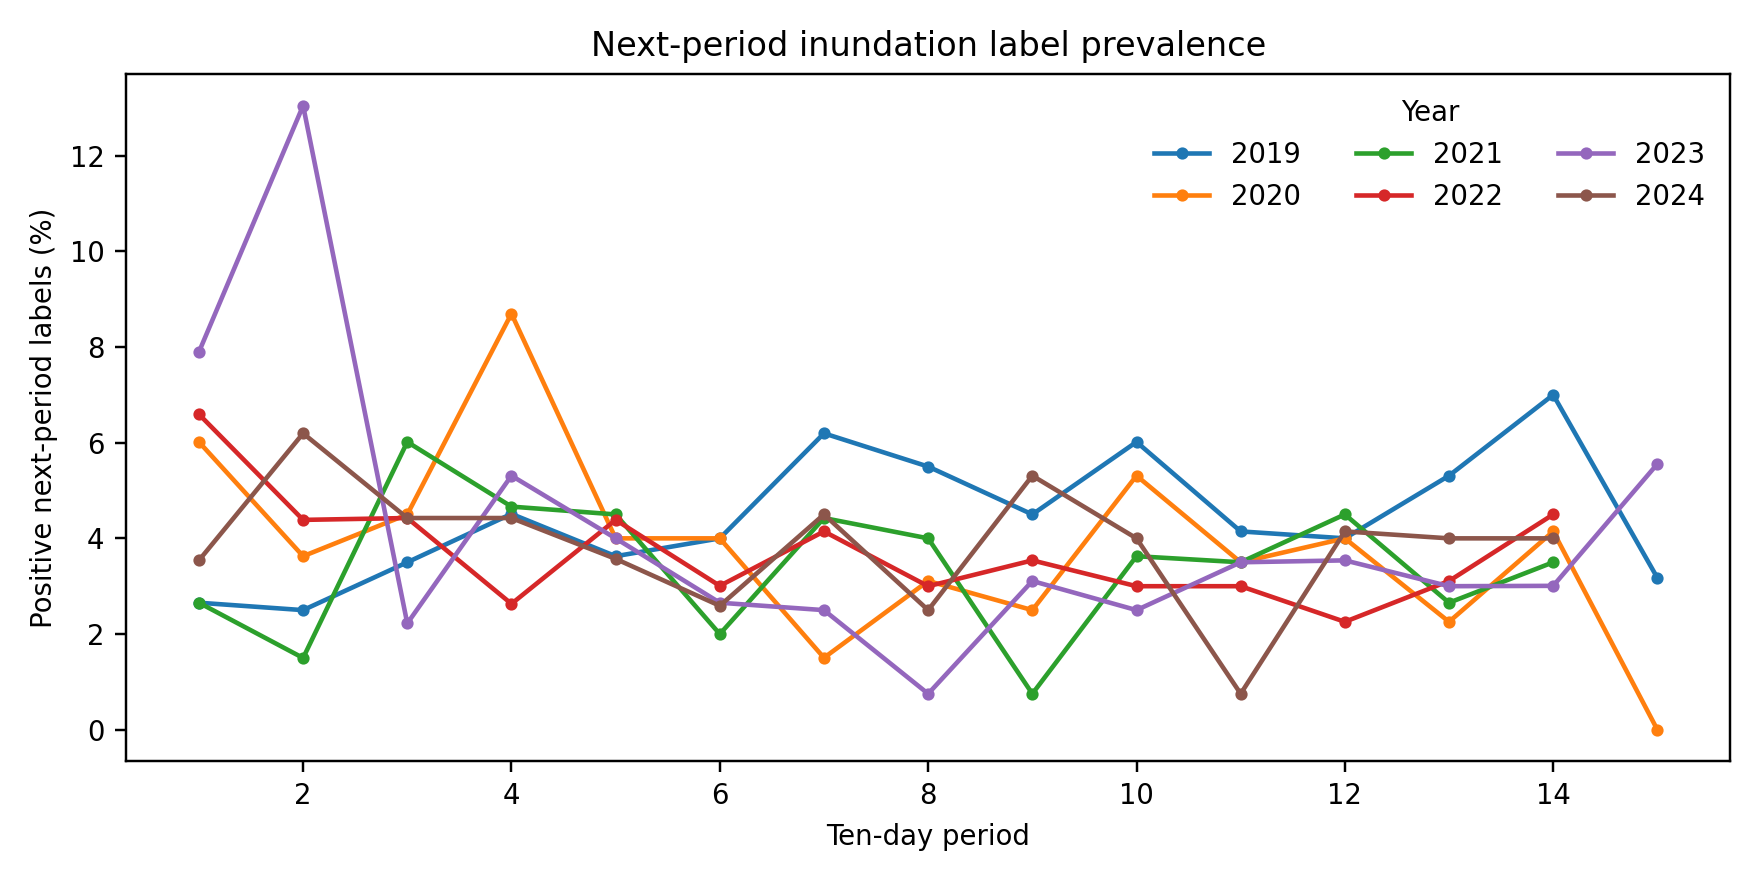
\includegraphics[width=\linewidth]{03_frequence_temporelle.png}
\end{minipage}
\caption{Data missingness among the most incomplete variables (left) and observed prevalence of the next-period inundation target by ten-day period and year (right). The prevalence denominator includes only rows with a valid target.}
\label{fig:coverage-prevalence}
\end{figure}

\subsection{Multiyear inundation dynamics}
Across the 96 exported annual-period records, three had no Sentinel-1 acquisition and are excluded from area means. Mean mapped area per valid period ranged from 128,213 ha in 2023 to 212,994 ha in 2019; the largest period-level estimate was 397,106 ha in 2021. The sum of valid period estimates is expressed as hectares-periods, not a unique seasonal footprint, because the same land can be counted repeatedly. Target prevalence varied from 3.47\% in 2021 to 4.41\% in 2019. Across all valid current labels, the mean sampled-point inundation frequency was 3.74\%; the median site frequency was zero. Frequencies are conditional on valid observations and the fixed sample, not unbiased estimates for every location in the valley.

For the next-period target, the strongest pairwise rank association among available predictors was with JRC maximum water extent (Spearman $\rho=0.287$); NDWI was positively associated ($\rho=0.153$), while NDVI, EVI, and MSAVI associations were negative (absolute $\rho$ approximately 0.160--0.163). The dry-reference water indicator was also associated with the target ($\rho=-0.234$), but is excluded from the primary model because it contributes to target construction. These coefficients are descriptive and not causal; inferential p-values are nominal with respect to repeated-site dependence.

\begin{table}[t]
\centering
\caption{Period-level mapped inundated area (100-m export), next-period target prevalence, and Sentinel-1 coverage by year. Area values are not unique seasonal totals; mean acquisition count is calculated over periods with at least one image.}
\label{tab:annual-flood}
\begin{tabular}{rrrrrrr}
\toprule
Year & Valid target $n$ & Flood target (\%) & Valid S1 periods & Mean S1 images & Mean/period (ha) & Max/period (ha) \\
\midrule
2019 & 2,517 & 4.41 & 16 & 4.875 & 212,994 & 339,014 \\
2020 & 2,337 & 3.72 & 16 & 4.500 & 148,678 & 300,576 \\
2021 & 2,391 & 3.47 & 15 & 5.067 & 193,367 & 397,106 \\
2022 & 2,111 & 3.60 & 15 & 4.667 & 152,495 & 220,249 \\
2023 & 2,115 & 3.50 & 16 & 4.312 & 128,213 & 190,107 \\
2024 & 2,112 & 3.79 & 15 & 4.533 & 136,592 & 276,264 \\
\bottomrule
\end{tabular}
\end{table}

\begin{figure}[t]
\centering
\begin{minipage}{0.48\linewidth}\centering
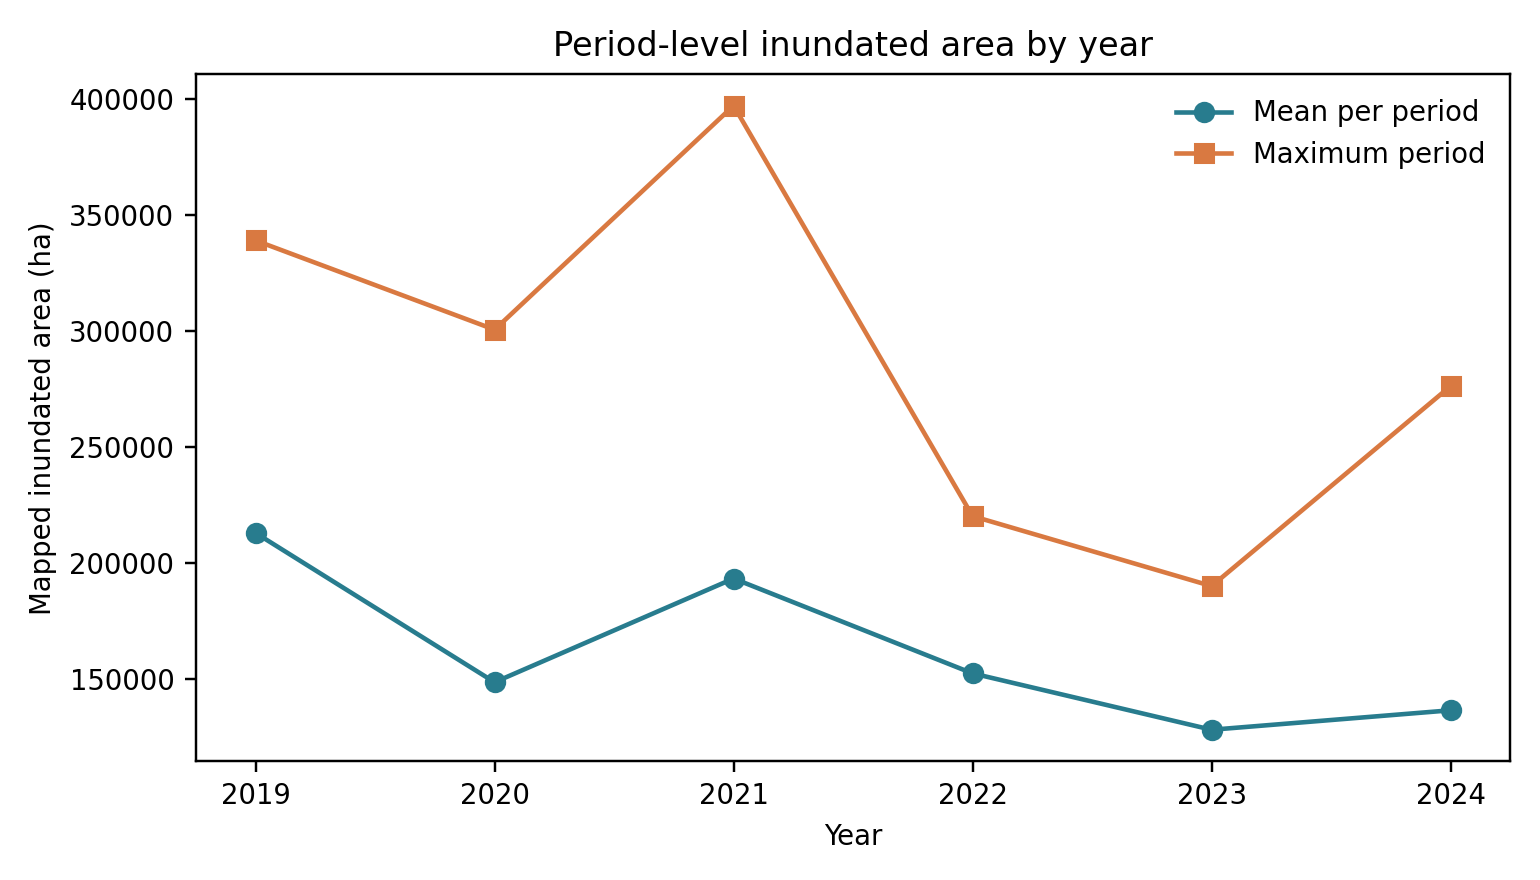
\includegraphics[width=\linewidth]{02_superficie_annuelle.png}
\end{minipage}\hfill
\begin{minipage}{0.48\linewidth}\centering
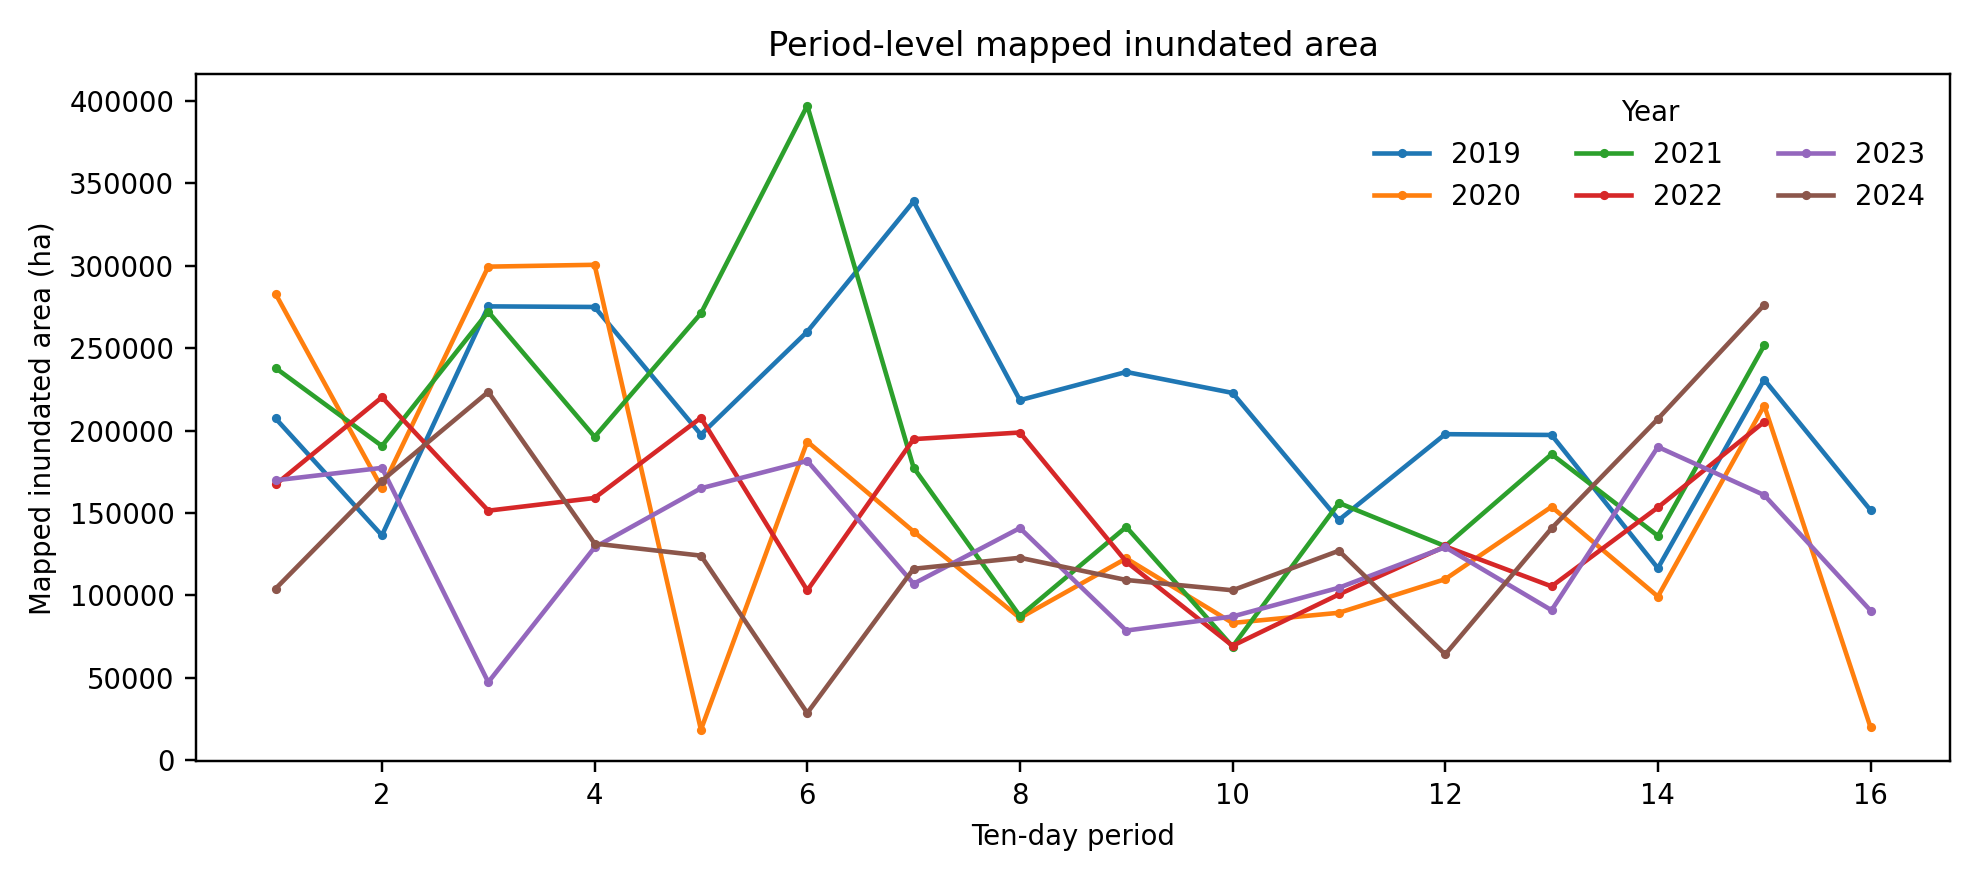
\includegraphics[width=\linewidth]{05_superficie_par_periode.png}
\end{minipage}
\caption{Area summaries derived from the six 100-m period-level CSV exports: annual mean and maximum over periods with Sentinel-1 observations (left), and ten-day trajectories (right). These are mapped potential-inundation estimates, not field-validated flood extents.}
\label{fig:flood-area}
\end{figure}

\subsection{Model comparison and spatial validation}
The 2019--2023 training data contain 11,471 valid next-period labels, including 431 positives. Among the five classifiers, Random Forest has the highest mean spatial-fold average precision (0.220, SD 0.214), followed by CatBoost (0.192, SD 0.178), XGBoost (0.161, SD 0.136), and logistic regression (0.140, SD 0.144). However, the persistence reference exceeds every classifier (AP 0.240, SD 0.125); the historical site-frequency reference for held-out sites reduces to the training prevalence baseline (AP 0.036, SD 0.019). Random Forest's mean Brier score (0.038) is also worse than the prevalence baseline (0.035). Fold variability is substantial, including one validation block with only 33 positives, so the classifier ranking is unstable and does not demonstrate skill beyond persistence.

\begin{table}[t]
\centering
\caption{Five-fold spatial validation on 2019--2023. Values are mean (standard deviation) across the five held-out coordinate clusters.}
\label{tab:spatial-validation}
\small
\begin{tabular}{lrrrr}
\toprule
Model & AP & AUC & Bal. acc. & Brier \\
\midrule
Persistence & 0.240 (0.125) & 0.745 (0.054) & 0.686 (0.053) & 0.033 (0.009) \\
Prevalence / unseen-site frequency & 0.036 (0.019) & 0.500 (0.000) & 0.500 (0.000) & 0.035 (0.018) \\
Balanced logistic regression & 0.140 (0.144) & 0.680 (0.119) & 0.621 (0.089) & 0.227 (0.071) \\
Balanced Random Forest & 0.220 (0.214) & 0.797 (0.065) & 0.556 (0.080) & 0.038 (0.013) \\
XGBoost & 0.161 (0.136) & 0.764 (0.072) & 0.608 (0.099) & 0.107 (0.093) \\
CatBoost & 0.192 (0.178) & 0.792 (0.077) & 0.612 (0.105) & 0.092 (0.078) \\
\bottomrule
\end{tabular}
\end{table}

\begin{figure}[t]
\centering
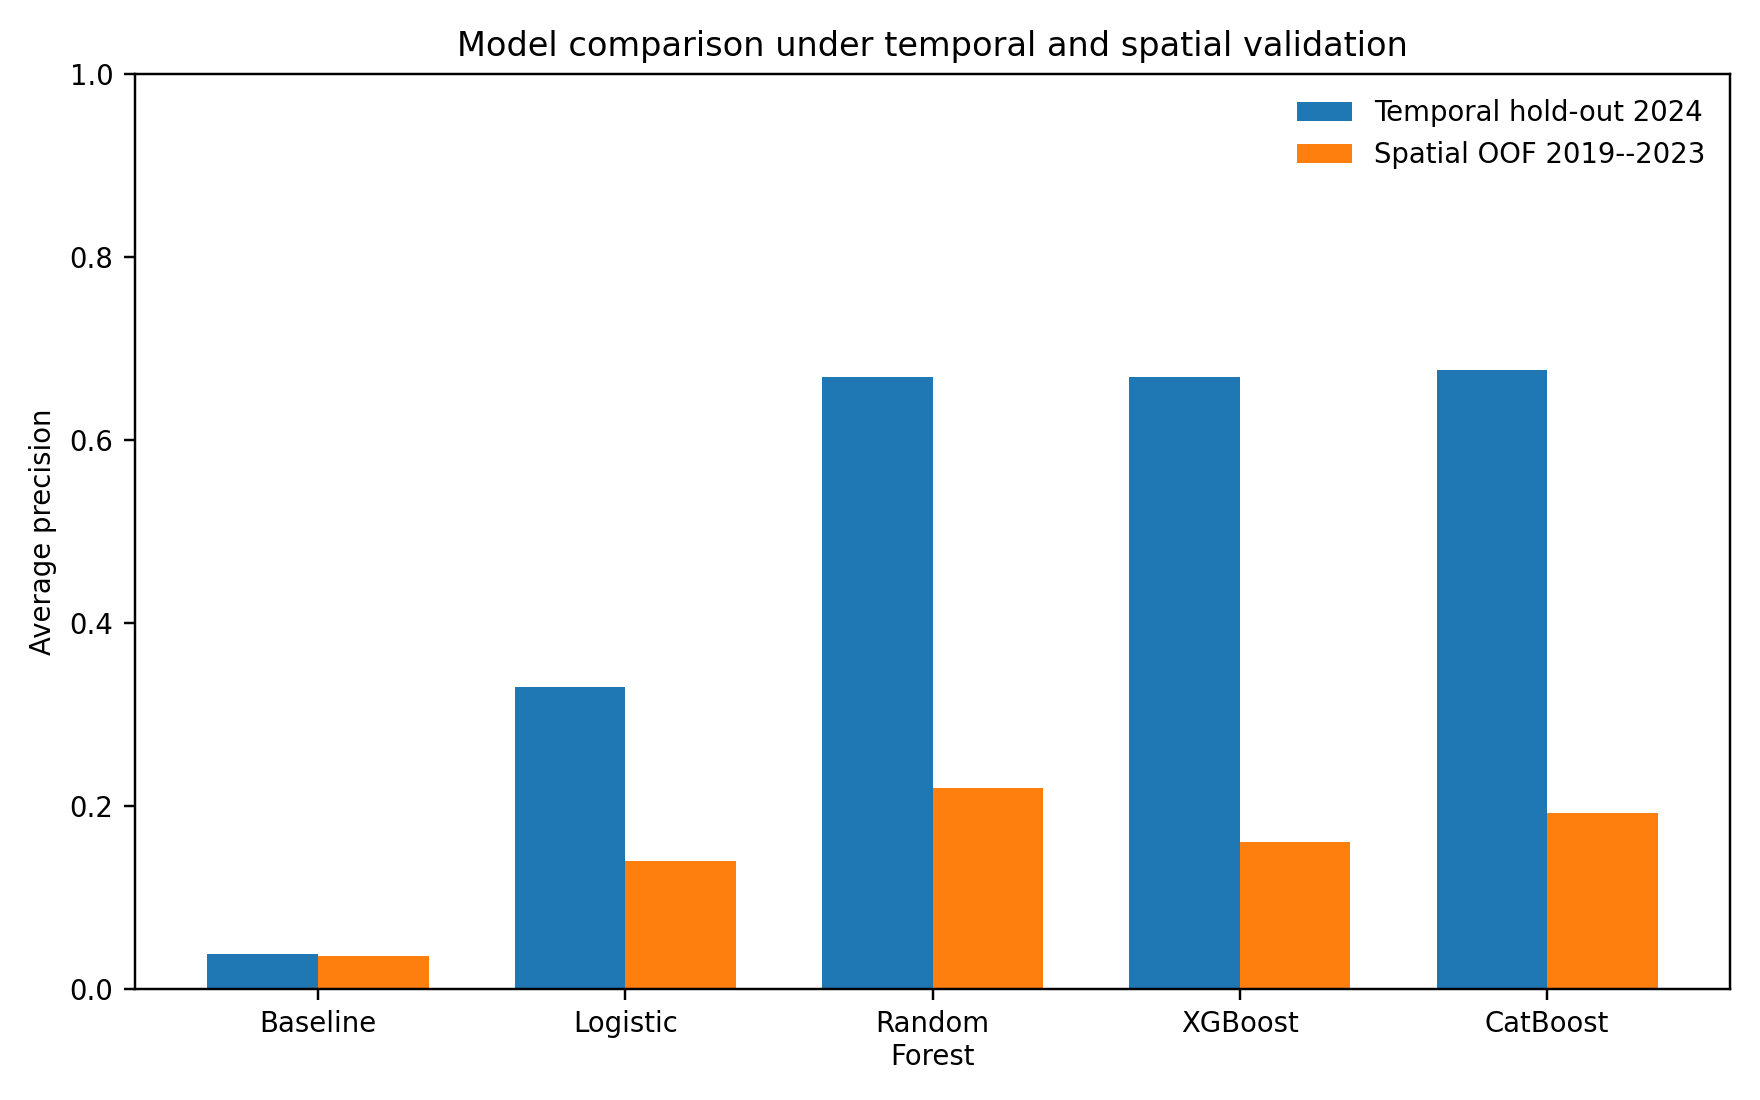
\includegraphics[width=0.78\linewidth]{09_comparaison_modeles.png}
\caption{Average precision for the five classifier candidates under site-grouped spatial validation and the 2024 temporal hold-out. Simple-reference scores, including persistence, are reported in Tables~\ref{tab:spatial-validation} and~\ref{tab:baselines}. The 2024 scores were not used for model selection.}
\label{fig:model-comparison}
\end{figure}

\subsection{Agricultural exposure}
Six numeric annual agricultural CSV exports provide 96 ten-day summaries at 10-m calculation scale. Three periods have no Sentinel-1 acquisitions (one each in 2021, 2022, and 2024); their area outcomes are treated as missing, not zero. Across the 93 valid periods, estimated mean potentially inundated candidate agricultural area per period ranges from 1,936 ha in 2020 to 8,827 ha in 2021, and the maximum single-period estimate is 15,724 ha in 2021. The fraction of radar-observed candidate agricultural area classified as inundated, pooled across valid periods within each year, ranges from 1.76\% (2020) to 4.17\% (2021). The corresponding mean period-level estimates are 7,847 ha (2019), 1,936 ha (2020), 8,827 ha (2021), 2,996 ha (2022), 7,283 ha (2023), and 3,334 ha (2024). These are threshold- and mask-dependent potential exposure estimates, not confirmed crop damage. The 10-m agricultural-exposure exports are not directly interchangeable with the separate 100-m flood-area exports in Table~\ref{tab:annual-flood}.

\begin{table}[t]
\centering
\caption{Potential exposure of general candidate agricultural surfaces from 10-m annual exports. Estimates exclude periods with no Sentinel-1 acquisition. The pooled percentage is exposed area divided by radar-observed candidate agricultural area across valid periods; hectare-period sums are not unique seasonal footprints.}
\label{tab:crop-exposure}
\small
\begin{tabular}{rrrrr}
\toprule
Year & Valid periods & Mean exposed (ha/period) & Maximum (ha) & \makecell{Pooled observed\\agricultural area\\exposed (\%)}\\
%Pooled observed agricultural area exposed (\%) \\
\midrule
2019 & 16 & 7,847 & 12,297 & 3.92 \\
2020 & 16 & 1,936 & 3,748 & 1.76 \\
2021 & 15 & 8,827 & 15,724 & 4.17 \\
2022 & 15 & 2,996 & 4,965 & 2.63 \\
2023 & 16 & 7,283 & 11,777 & 3.73 \\
2024 & 15 & 3,334 & 8,626 & 3.25 \\
\bottomrule
\end{tabular}
\end{table}

\begin{figure}[t]
\centering
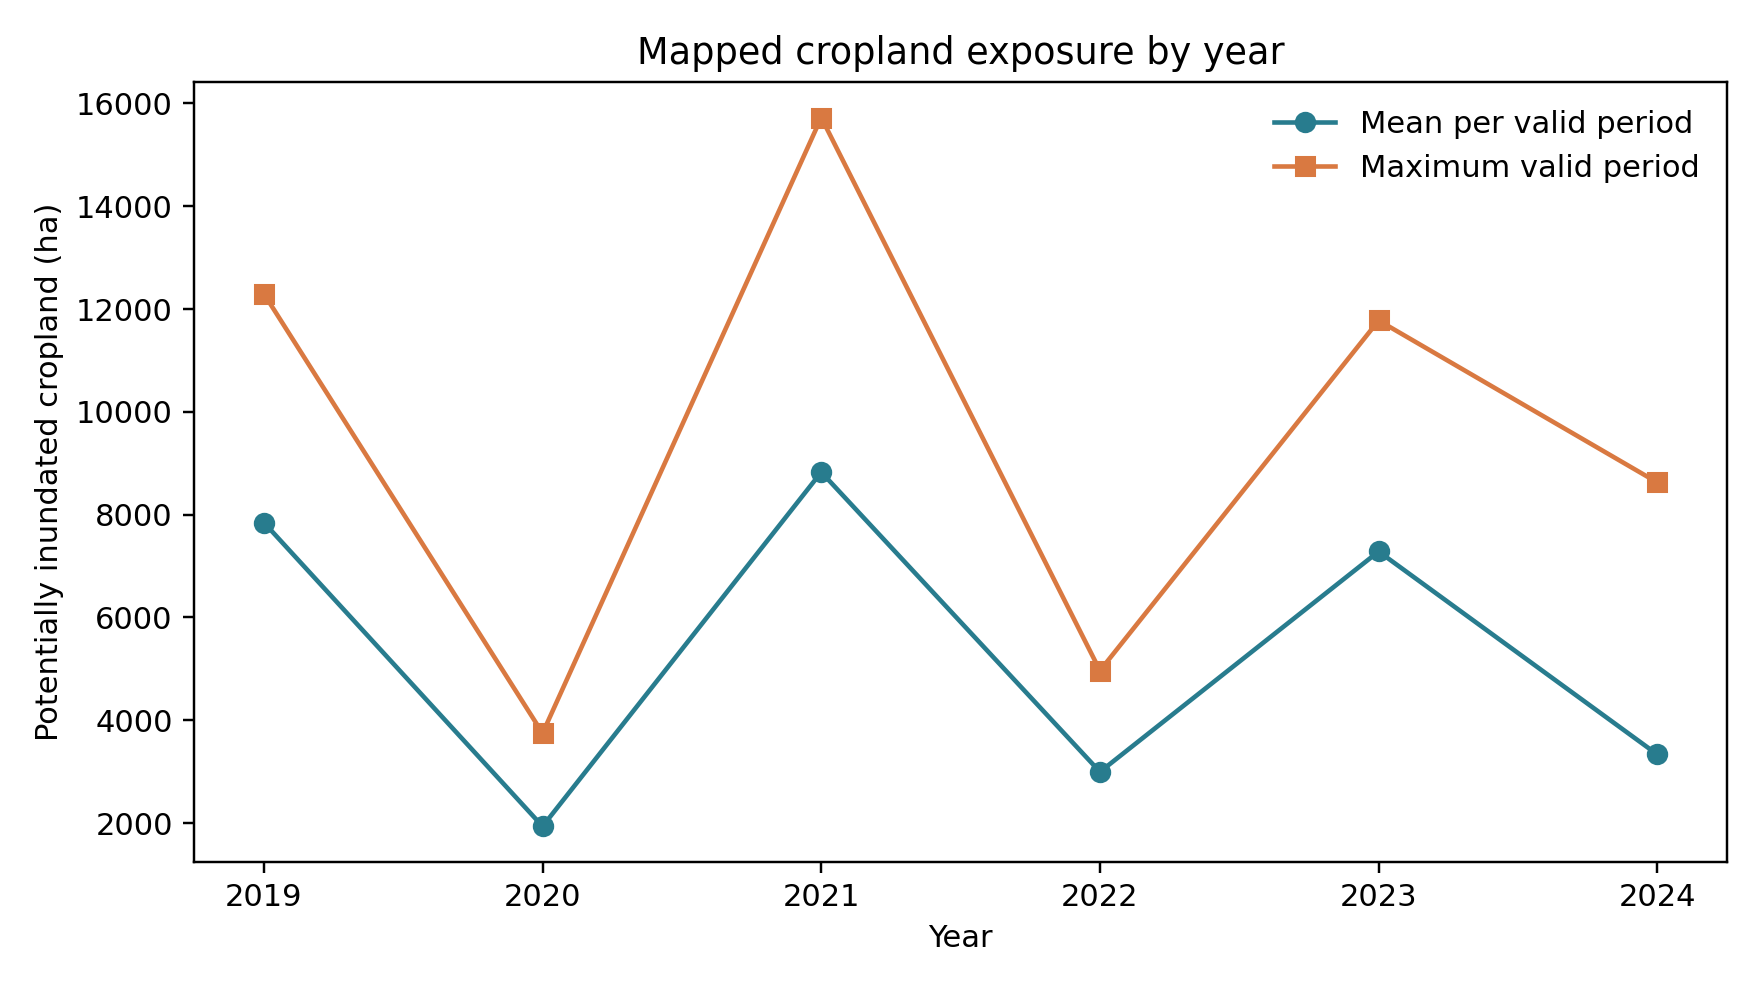
\includegraphics[width=0.76\linewidth]{12_exposition_agricole.png}
\caption{Mean and maximum potentially inundated candidate agricultural area per valid ten-day period, estimated from the 10-m exposure exports.}
\label{fig:crop-exposure}
\end{figure}

The point-level frequency map in Fig.~\ref{fig:frequency-model} shows sampled flood recurrence only; it is not a crop-specific damage map. This study reports no crop-type classification, observed destruction, yield reduction, household income, or farmer economic loss. The rice examples in Methods are hypothetical sensitivity calculations and are not empirical findings for any year or location in the valley.

\begin{figure}[t]
\centering
\begin{minipage}{0.48\linewidth}\centering
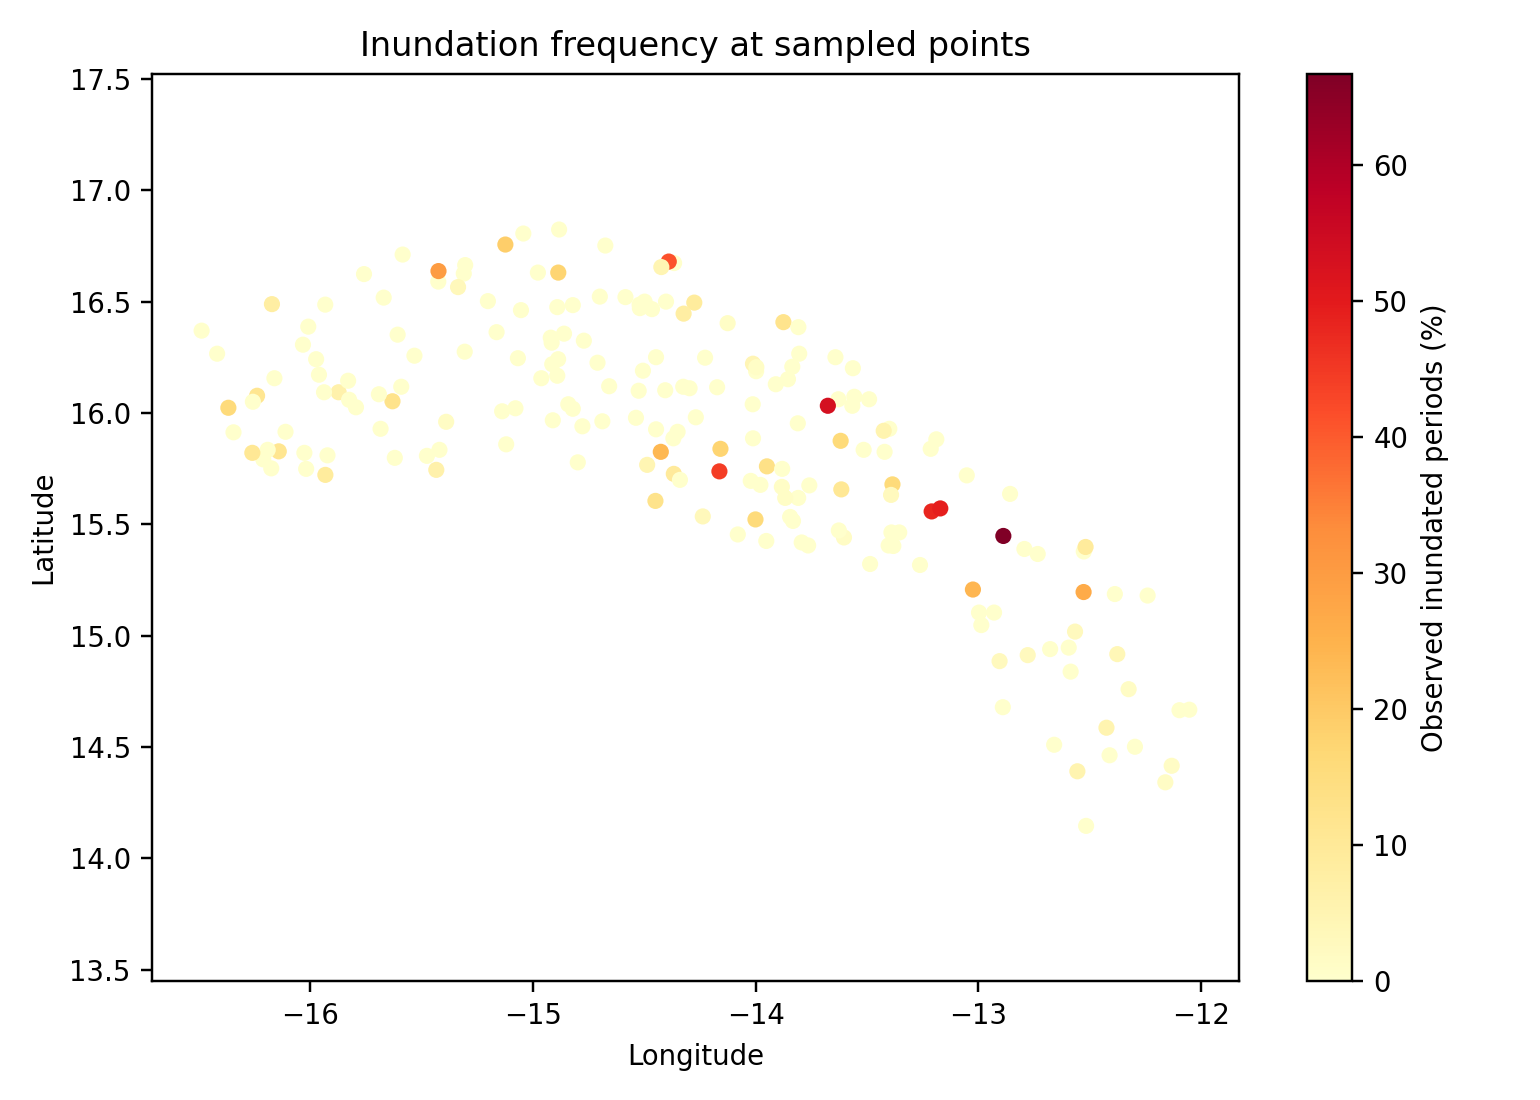
\includegraphics[width=\linewidth]{04_frequence_spatiale_points.png}
\end{minipage}\hfill
\begin{minipage}{0.48\linewidth}\centering
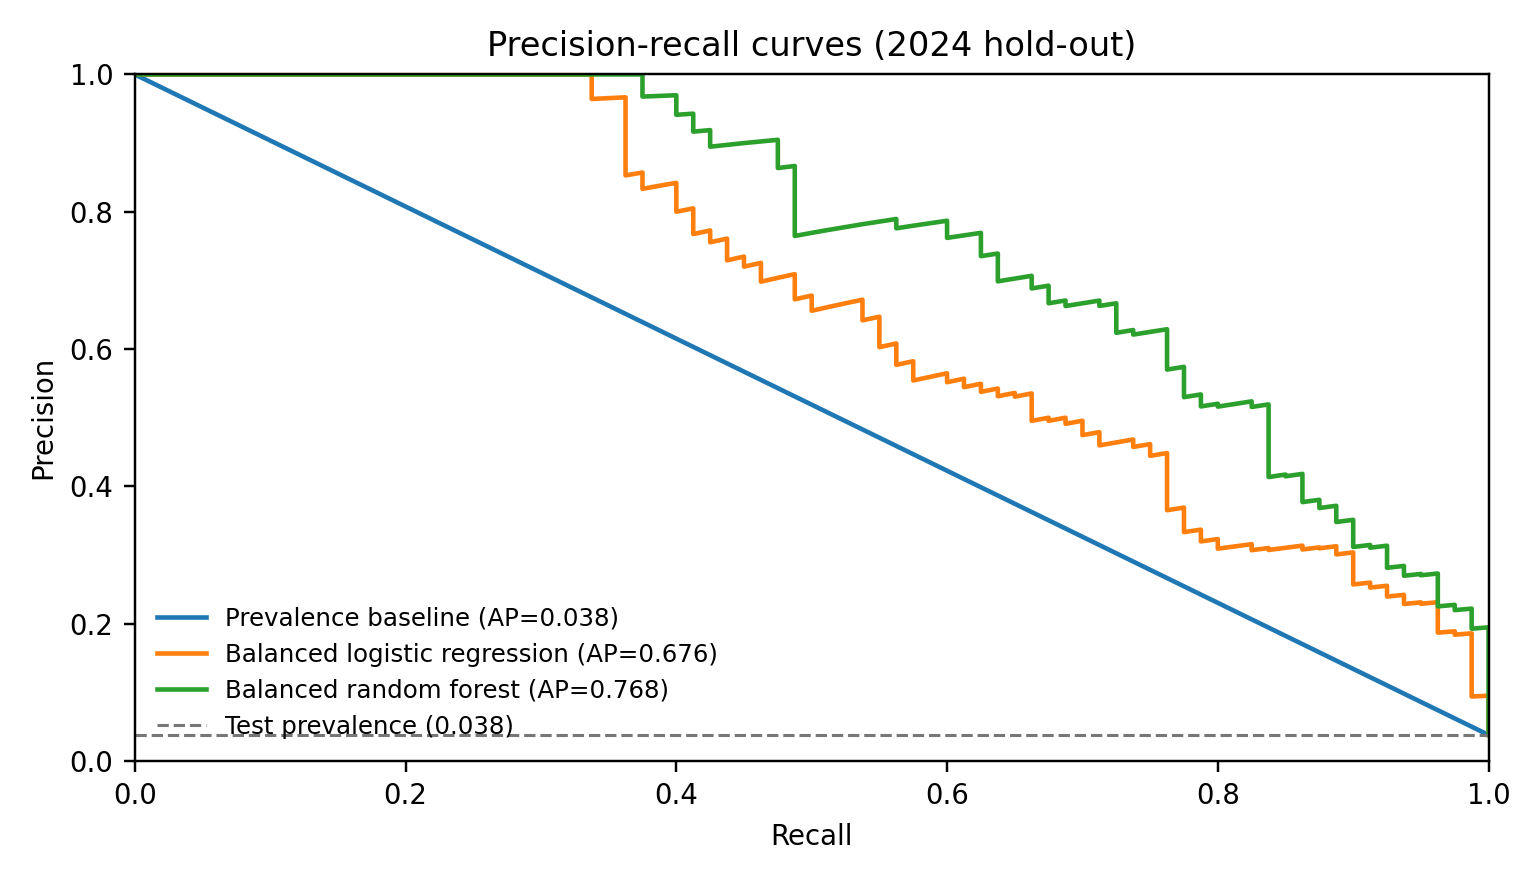
\includegraphics[width=\linewidth]{06_modeles_precision_rappel_2024.png}
\end{minipage}
\caption{Observed recurrence at the 200 sampled sites (left; valid periods only) and precision--recall curves for the held-out 2024 next-period classification task (right).}
\label{fig:frequency-model}
\end{figure}

\subsection{Prediction performance}
Training used 11,471 labeled records from 2019--2023; the 2024 temporal test contains 2,112 records, including 80 positives. The spatial ranking among the three leading machine-learning candidates is Random Forest (AP 0.220, SD 0.214), CatBoost (0.192, SD 0.178), and XGBoost (0.161, SD 0.136). The large fold-to-fold variability makes this ranking uncertain. On the 2024 temporal hold-out, Random Forest has AP 0.669, but the historical site-frequency reference reaches 0.494 and persistence reaches 0.333; this test reuses training sites and is not the primary transfer result.

\begin{table}[t]
\centering
\caption{Exploratory model performance on the 2024 chronological hold-out set. The classification threshold is 0.5; average precision is the principal ranking metric under class imbalance.}
\label{tab:model-performance}
\small
\begin{tabular}{lrrrrrrr}
\toprule
Model & Prec. & Recall & F1 & Bal. acc. & AUC & AP & Brier \\
\midrule
Prevalence baseline & 0.000 & 0.000 & 0.000 & 0.500 & 0.500 & 0.038 & 0.036 \\
Balanced logistic regression & 0.070 & 0.738 & 0.129 & 0.677 & 0.810 & 0.330 & 0.228 \\
Balanced Random Forest & 0.868 & 0.413 & 0.559 & 0.705 & 0.943 & 0.669 & 0.023 \\
XGBoost & 0.296 & 0.825 & 0.436 & 0.874 & 0.953 & 0.669 & 0.057 \\
CatBoost & 0.368 & 0.713 & 0.485 & 0.832 & 0.952 & 0.677 & 0.045 \\
\bottomrule
\end{tabular}
\end{table}

\begin{table}[t]
\centering
\caption{Simple-reference and feature-ablation results. Scores are computed on the same 2024 records; the joint space--time test uses the same held-out blocks as the leading Random Forest classifier.}
\label{tab:baselines}
\small
\begin{tabular}{llrrr}
\toprule
Evaluation & Method & AP & ROC-AUC & Brier \\
\midrule
2024 temporal & Prevalence baseline & 0.038 & 0.500 & 0.036 \\
2024 temporal & Persistence & 0.333 & 0.786 & 0.031 \\
2024 temporal & Historical site frequency & 0.494 & 0.939 & 0.025 \\
2024 temporal & Random Forest & 0.669 & 0.943 & 0.023 \\
2024 space--time & Prevalence for unseen sites & 0.038 & 0.500 & 0.036 \\
2024 space--time & Persistence & 0.333 & 0.786 & 0.031 \\
2024 space--time & Random Forest & 0.379 & 0.835 & 0.037 \\
2024 space--time & Random Forest without contemporaneous Sentinel-1 & 0.202 & 0.739 & 0.049 \\
\bottomrule
\end{tabular}
\end{table}

\noindent\textbf{Joint space--time test.} When 2024 sites are predicted only by models that excluded their entire spatial block from 2019--2023 training, the leading Random Forest classifier obtains precision 0.750, recall 0.263, F1 0.389, balanced accuracy 0.630, ROC-AUC 0.835, average precision 0.379, and Brier score 0.037 on the 2,112 test records (80 positive). The lower average precision than the temporal-only score (0.669) quantifies the cost of transferring to both a future year and withheld locations.

\noindent\textbf{Label-proxy ablation.} For the leading Random Forest classifier, reintroducing \texttt{eau\_ref\_seche}, which contributes to label construction, raises mean spatial-fold average precision from 0.220 (SD 0.214) to 0.425 (SD 0.212) and temporal 2024 average precision from 0.669 to 0.757. The primary metrics and SHAP analysis therefore exclude this variable; the ablation demonstrates the inflation associated with a predictor that is not independent of the target definition.

\begin{figure}[t]
\centering
\begin{minipage}{0.48\linewidth}\centering
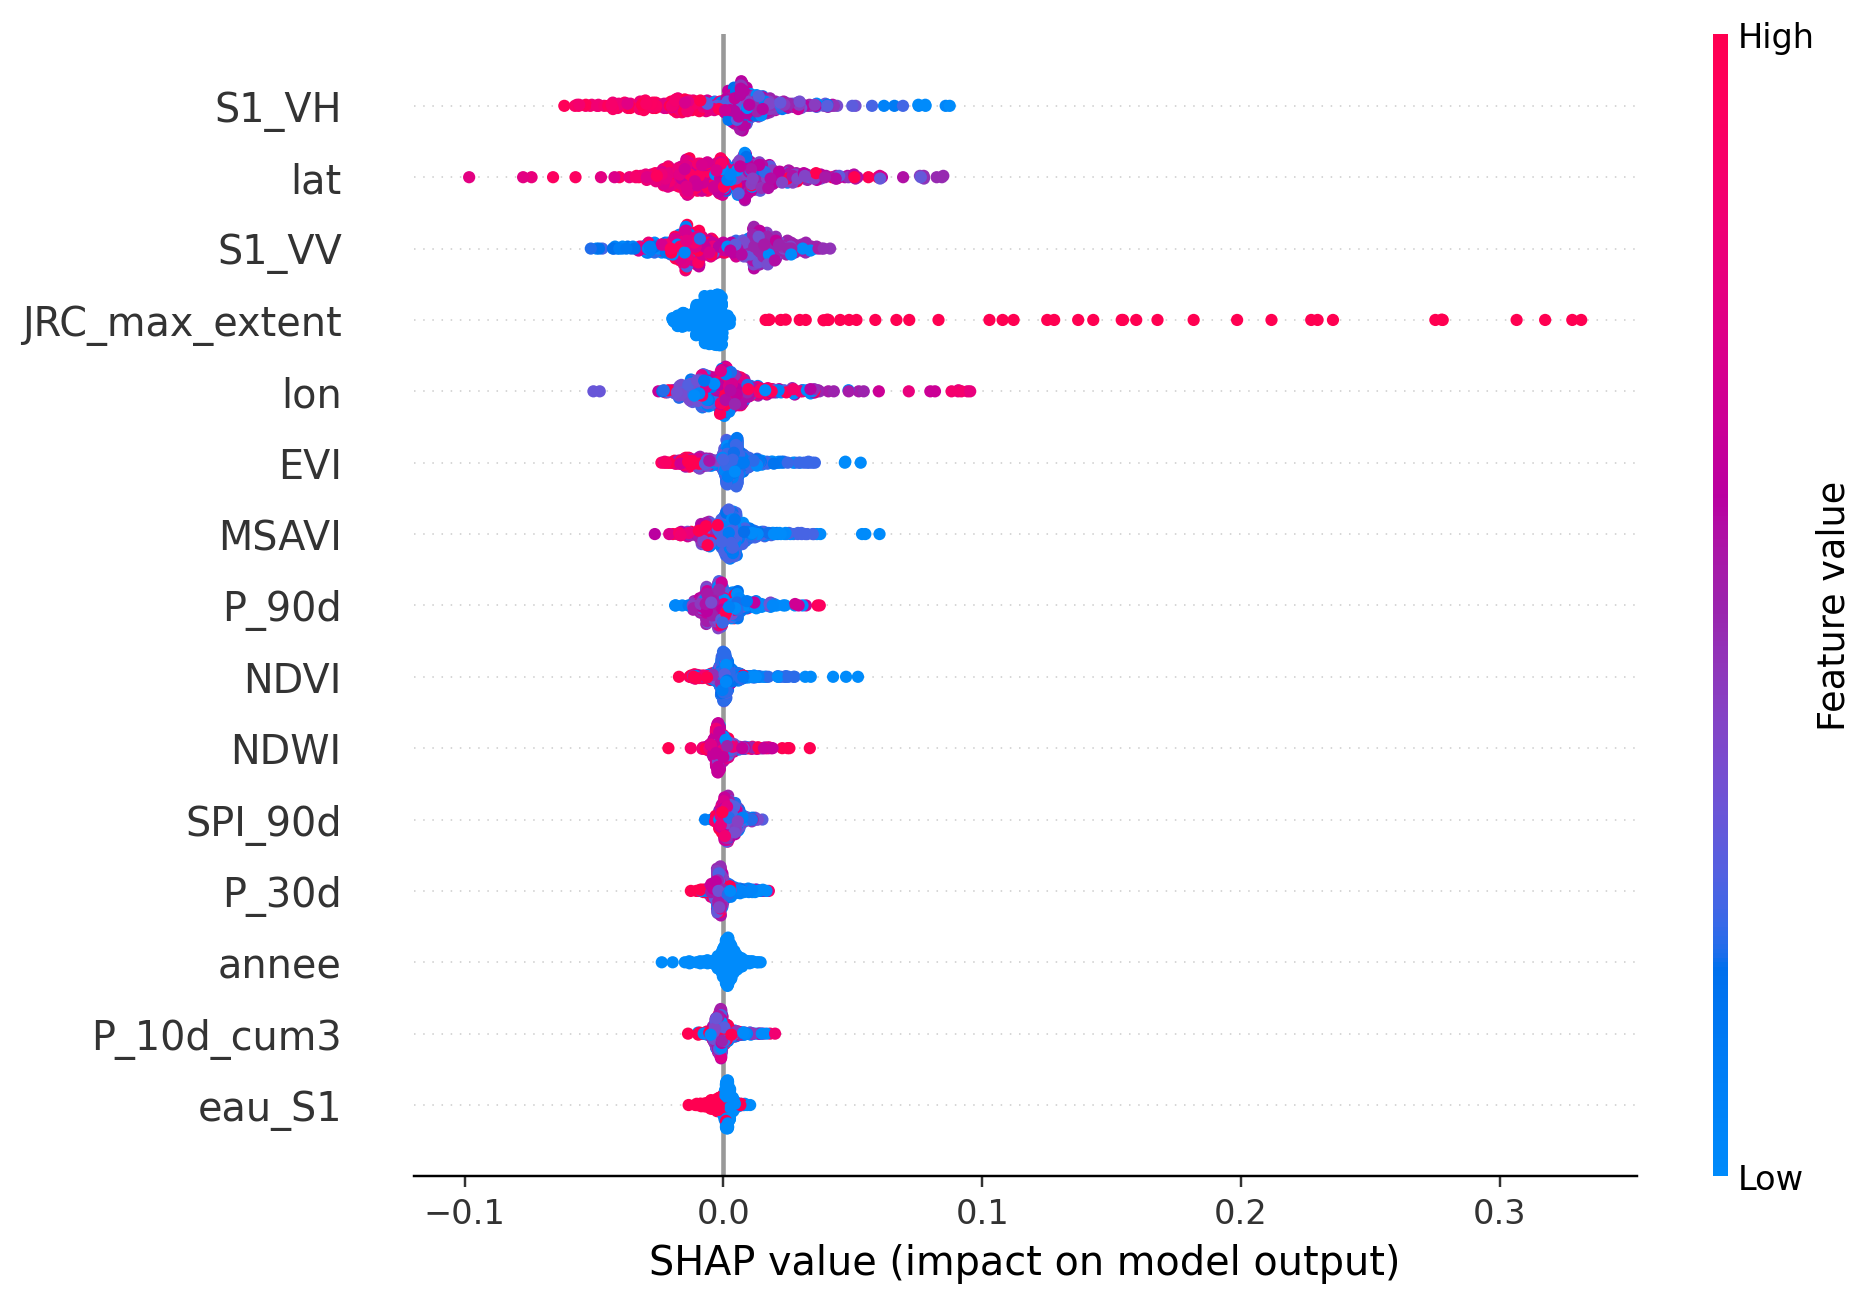
\includegraphics[width=\linewidth]{10_shap_summary.png}
\end{minipage}\hfill
\begin{minipage}{0.48\linewidth}\centering
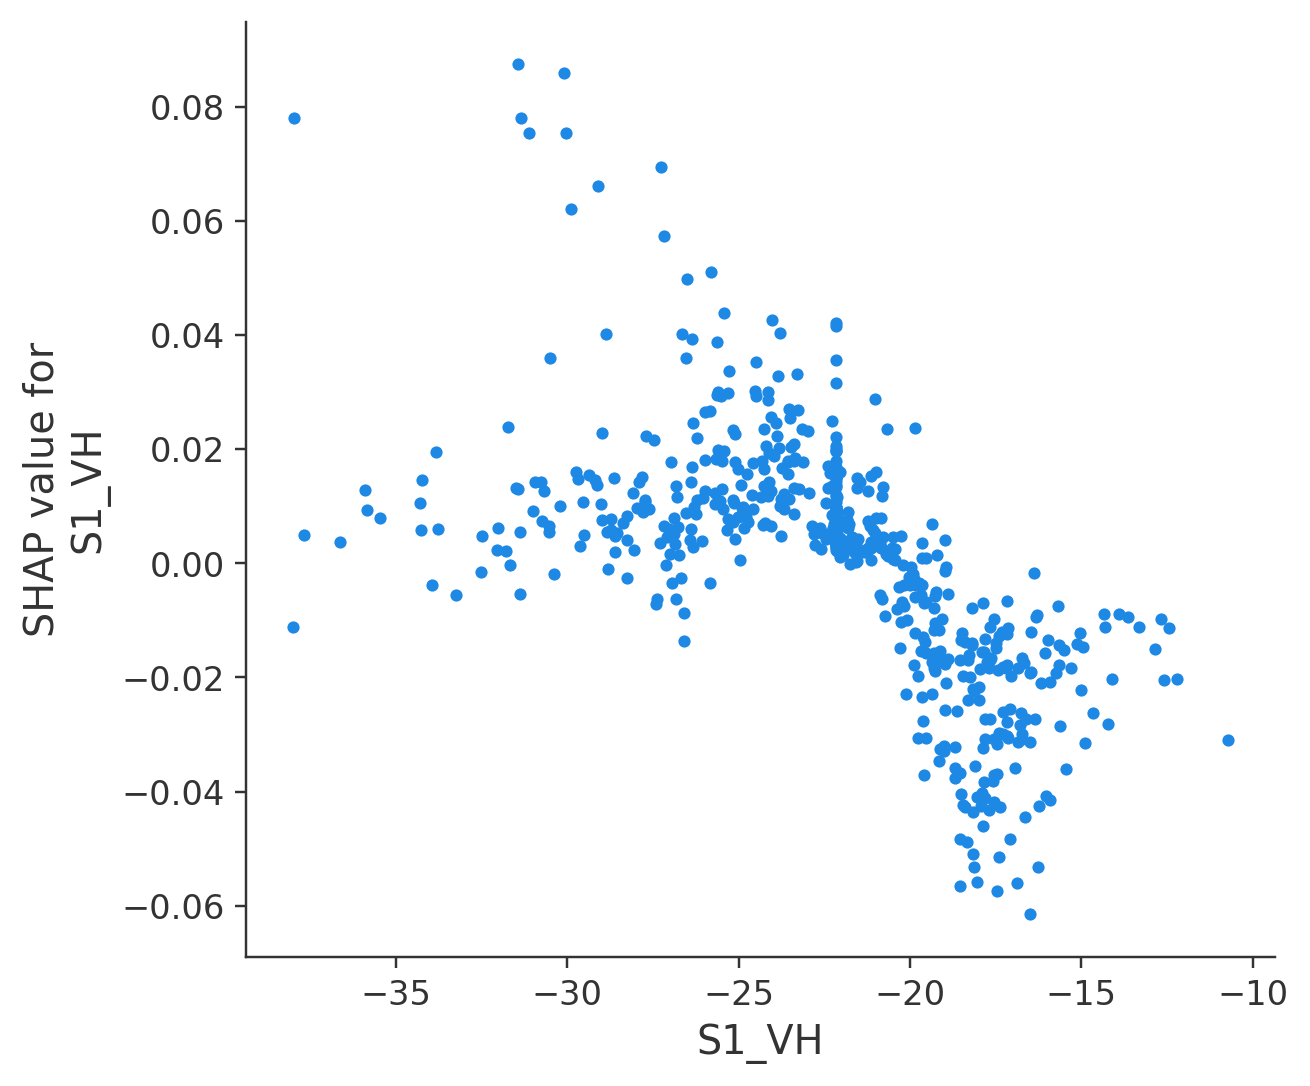
\includegraphics[width=\linewidth]{11_shap_dependance.png}
\end{minipage}
\caption{SHAP explanation of the selected Random Forest without the label-overlapping dry-reference indicator. The left panel ranks global mean absolute contributions; the right panel shows the dependence of the most influential predictor, Sentinel-1 VH. SHAP attributions describe model behavior, not causal effects.}
\label{fig:shap}
\end{figure}

The largest mean absolute SHAP contributions are for S1 VH (0.0160), latitude (0.0160), S1 VV (0.0157), and JRC maximum water extent (0.0154), followed by longitude and optical indices. The close contributions and the prominence of coordinates and historical water indicate that geography and spatially structured prevalence remain influential. Pearson and Spearman tests similarly identify JRC maximum extent as the strongest available association with the next-period target ($r=\rho=0.287$); correlations do not establish causal influence.

\subsection{Comparison with published state of the art}
The numerical comparison is contextual because label, spatial unit, lead time, and reference data differ. Nevo et al. report median inundation-extent F1 values of 0.69 under one-year cross-validation and 0.76 under leave-extreme-out testing for operational river-flood mapping; Nearing et al. report reliable forecasts of extreme river floods at up to five days lead time in ungauged watersheds relative to a global-system nowcast \cite{nevo2022,nearing2024}. Neither evaluates a ten-day, point-level Sentinel-1-derived binary label in the Senegal River Valley.

\begin{table}[t]
\centering
\caption{Contextual comparison with relevant published systems. Scores are not directly comparable across targets or reference data.}
\label{tab:sota}
\begin{tabular}{p{0.16\linewidth}p{0.22\linewidth}p{0.24\linewidth}p{0.17\linewidth}}
\toprule
Study & Prediction target & Validation and reported result & Relation to this study \\
\midrule
Nevo et al. (2022) & River stage and inundation extent at operational gauges & Year-held-out and leave-extreme-out; median inundation F1 0.69 and 0.76 & Gauge/event maps, not point-level next-dekad labels. \\
Nearing et al. (2024) & Extreme river floods in ungauged watersheds & Up to 5-day lead time; reliability comparable to or better than GloFAS nowcasts & Global hydrologic warnings, not satellite-derived point classification. \\
This study, spatial hold-out & Next-period Sentinel-1 proxy at 200 sites & 5-fold spatial AP 0.220 (SD 0.214); joint 2024 space--time AP 0.379 & Valley-specific, sparse sample; label is not independently validated. \\
\bottomrule
\end{tabular}
\end{table}

Accordingly, this work does not claim to outperform the global or operational state of the art. Its contribution is a documented multiyear point--period dataset, an explicit label-circularity test, spatial and temporal generalization results for this valley, and a reproducible analysis of candidate flood predictors. A direct performance claim would require common independent flood-event labels, matching lead times and spatial units, and a shared test protocol.

\section{Discussion}
The model results are sensitive to the validation design and predictor set. In spatial validation, persistence (AP 0.240, SD 0.125) exceeds all five classifiers; Random Forest is only the best classifier and has AP 0.220 (SD 0.214). Its mean Brier score is worse than that of the prevalence baseline. In the joint 2024 space--time test, Random Forest exceeds persistence in AP (0.379 versus 0.333), but again has a worse Brier score (0.037 versus 0.031), indicating that ranking skill does not imply better probability calibration. Its AP falls to 0.202 when contemporaneous Sentinel-1 inputs are removed, below persistence. Thus, apparent skill depends substantially on radar information related to the satellite-derived target; independent flood truth is needed to establish forecasting skill. The historical site-frequency reference performs strongly in the temporal test because sites recur, illustrating why that split is not a test of spatial transfer. SHAP attributions describe fitted-model behavior and may reflect geographic prevalence; they are not causal explanations. The agricultural CSVs allow a provisional numeric overlap estimate, but the Dynamic World crop mask and fixed VV threshold are not locally validated. Repeated-period area sums double-count locations, and exposure must not be interpreted as damage or monetary loss. The crop-loss equations offer a transparent framework for future crop-specific assessment, while the 1,500-ha rice scenarios merely demonstrate parameter sensitivity. Seasonal floods can also support recession agriculture or soil-water recharge; their net effect depends on crop, timing, duration, and the counterfactual production system. Published systems such as Nevo et al. and Nearing et al. predict different hydrological targets at different lead times, so their results are context only.

\section{Limitations}
The study starts in 2019 because no 2018 export was available. A fixed VV threshold and pre-season reference may misclassify smooth bare soil, permanent or seasonal water, and water beneath vegetation. Flood labels have not been independently validated. Dynamic World probabilities are not field-verified agricultural parcels, and the 0.30 threshold has not been tested for sensitivity. Three agricultural periods lack Sentinel-1 acquisitions; remaining observations may also vary in spatial coverage. The 10-m agricultural-exposure and 100-m flood-area calculations use different scales and should not be read as a single harmonized estimate. The 200-site sampling design was not documented in the available project files, so point statistics cannot support unbiased valley-wide estimates. The five spatial clusters have no buffer, the 2024 temporal test reuses sites, and the joint test contains only 80 positives. Correlation p-values treat repeated observations as independent and are therefore descriptive only. The SPI calculation is documented here according to the supplied implementation specification, but the original SPI GEE source is absent and independent code-level verification is not possible. The fixed 1991--2020 reference also includes 2020 data for some earlier sample dates. Model hyperparameters and classification thresholds were not tuned in nested spatial validation; probability calibration and uncertainty intervals were not assessed. The no-Sentinel-1 ablation shows limited transfer signal. The supplemental AgriSmart files contain synthetic augmentation provenance (SMOTE and Gaussian variation) and no yield or income outcome, so they were not joined to the satellite labels. The illustrative rice yield and paddy-price inputs remain unverified assumptions; crop-specific affected areas and destruction fractions are unavailable, so no observed annual production or monetary losses can be calculated. Seasonal inundation may be harmful or beneficial depending on crop and timing. The additional 2018 coverage, independent labels, spatial covariates, sensitivity tests, and field/economic outcomes require new data and analyses.

\section{Conclusion}
This analysis describes Sentinel-derived flood dynamics and provisional exposure of general candidate agricultural surfaces for 2019--2024 in the Senegal River Valley. Random Forest is the best of five classifiers but is outperformed by persistence in spatial validation; it exceeds persistence only in the joint 2024 test, where probability error remains worse. Removing contemporaneous Sentinel-1 predictors reduces its joint-test AP to 0.202. The agricultural exports estimate 1,936--8,827 ha of potentially inundated candidate agricultural area per valid ten-day period depending on year, but these satellite overlaps are not validated damage or economic losses. A conditional loss method and hypothetical sensitivity scenarios are provided in Methods; annual losses remain unestimated because crop-specific affected area, destruction fraction, and locally verified yield and paddy price are absent. Independent flood labels, local agricultural-mask validation, documented sampling, hydrological/topographic predictors, and field yield or household-economic data are needed before operational or livelihood-impact claims can be made.

\backmatter

\section*{Declarations}
\subsection*{Acknowledgements}
The authors thank Universit\'e Alioune Diop de Bambey and the UFR SATIC Department of Information and Communication Technologies (TIC) for institutional support. Pape El Hadji Abdoulaye Gueye carried out the study under the scientific review and supervision of his co-authors and senior supervisors at UFR SATIC.

\subsection*{Funding}
This research received no external funding.

\subsection*{Competing interests}
The authors declare no competing interests.

\subsection*{Data availability}
The tabular project data, analysis code, derived tables, model predictions, correlation outputs, SHAP values, exposure summaries, scenario calculations, and figures are available from \url{https://github.com/papegu/Analyse_prediction_innondations_vallee_fleuve_senegal}. The original GeoTIFF flood and agricultural-exposure map tiles are hosted in the Google Drive folder \url{https://drive.google.com/drive/u/0/folders/18wlX2CnwW32UaeEAWIWh0rnxVra63mLH}. Access to that folder depends on its Google Drive sharing settings; the authors must enable link access or otherwise provide access for readers before publication. Source satellite products and Earth Engine assets remain subject to their respective access conditions.

\subsection*{Code availability}
All analysis scripts, including the GEE agricultural-exposure export and the Python processing and modeling workflows, are archived with the tabular data at \url{https://github.com/papegu/Analyse_prediction_innondations_vallee_fleuve_senegal}. The SPI-generation source was not present in the project files at the time of this revision and should be added to the repository when available.

\subsection*{Author contributions}
Pape El Hadji Abdoulaye Gueye performed the data processing, GEE and statistical analyses, model development, and initial manuscript drafting. Cherif Bachir Deme, Adrien Basse, and Diery Ngom provided scientific supervision, methodological review, and critical manuscript revision as senior supervisors at UFR SATIC, Department of Information and Communication Technologies (TIC). All authors reviewed and approved the final manuscript.

\bibliography{references}

\end{document}
